\documentclass[12pt,a4paper]{report}
\usepackage[a4paper,left=1.5in,right=1in,top=1in,bottom=1in]{geometry}
\usepackage{times}
\usepackage[T1]{fontenc}
\usepackage{graphicx}
\usepackage{grffile}
\usepackage{booktabs}
\usepackage{tabularx}
\usepackage{setspace}
\usepackage{titlesec}
\usepackage{fancyhdr}
\usepackage{enumitem}
\usepackage[hidelinks]{hyperref}
\usepackage{caption}
\captionsetup[figure]{labelfont=bf,font=small}
\captionsetup[table]{labelfont=bf,font=small}
\onehalfspacing
\titleformat{\chapter}[display]
  {\centering}{\large\bfseries CHAPTER \thechapter}{6pt}{\Large\bfseries}
\titlespacing*{\chapter}{0pt}{0pt}{24pt}
\pagestyle{fancy}
\fancyhf{}
\fancyfoot[R]{Page \textbar\ \thepage}
\renewcommand{\headrulewidth}{0pt}

\title{}
\author{}
\date{}

\begin{document}

% ============================================================= TITLE PAGE
\begin{titlepage}
\begin{center}
\vspace*{2cm}
\parbox{0.85\linewidth}{\centering\bfseries\Large Consistency-Preserving Adversarial Robustness and SHAP-Guided Hybrid Defence for Flow-Based Network Intrusion Detection}\\[0.6cm]
A Minor Project Thesis\\[0.5cm]
Submitted in partial fulfillment of the requirements for the award of the Degree of\\[0.4cm]
{\bfseries\large BACHELOR OF TECHNOLOGY}\\[0.2cm]
in\\[0.2cm]
{\bfseries COMPUTER SCIENCE AND ENGINEERING}\\[0.8cm]
By\\[0.3cm]
{\bfseries\large Shreyanka Basak\ \ (BTECH/15115/24)}\\[0.2cm]
{\bfseries\large Aditi Maharor\ \ (BTECH/15173/24)}\\[0.8cm]
Under the guidance of\\[0.2cm]
{\bfseries Dr. Subhash Chandra Pandey}\\
Assistant Professor\\[0.8cm]

\includegraphics[width=1.3in]{assets/logo_candidate_0.png}\\[0.8cm]
{\bfseries DEPARTMENT OF COMPUTER SCIENCE AND ENGINEERING}\\
{\bfseries BIRLA INSTITUTE OF TECHNOLOGY, MESRA}\\
{\bfseries OFF-CAMPUS PATNA -- 800014}\\[0.3cm]
CS24300 --- Minor Project
\end{center}
\end{titlepage}

% ============================================================= APPROVAL OF GUIDE
\begin{center}\bfseries\Large Approval of the Guide\end{center}
\vspace{0.5cm}
Recommended that the project entitled \textit{``Consistency-Preserving Adversarial Robustness and SHAP-Guided Hybrid Defence for Flow-Based Network Intrusion Detection''} presented by Shreyanka Basak (BTECH/15115/24) and Aditi Maharor (BTECH/15173/24) under my supervision and guidance be accepted as fulfilling this part of the requirements for the award of the Degree of Bachelor of Technology in Computer Science and Engineering. To the best of my knowledge, the content of this project did not form a basis for the award of any previous degree to anyone else.
\vspace{2cm}

\noindent Date: \hrulefill \hfill \hrulefill \\
\hfill \textbf{Dr. Subhash Chandra Pandey}\\
\hfill Assistant Professor, Designation: \hrulefill

\vspace{1cm}
\begin{center}
Department of Computer Science and Engineering\\
Birla Institute of Technology, Mesra, Off-Campus Patna
\end{center}
\vspace{2cm}
\begin{center}
\hrulefill\\
Head of the Department\\
Department of Computer Science and Engineering\\
Birla Institute of Technology, Mesra, Off-Campus Patna
\end{center}
\newpage

% ============================================================= DECLARATION CERTIFICATE
\begin{center}\bfseries\Large Declaration Certificate\end{center}
\vspace{0.5cm}
We certify that
\begin{enumerate}[label=(\alph*)]
\item the work contained in this project is original and has been done by us under the general supervision of our supervisor;
\item the work has not been submitted to any other Institute for any other degree or diploma;
\item we have followed the guidelines provided by the Institute in writing the report;
\item we have conformed to the norms and guidelines given in the Ethical Code of Conduct of the Institute;
\item whenever we have used materials (data, theoretical analysis, figures and text) from other sources, we have given due credit to them by citing them in the text of the report and giving their details in the references; and
\item whenever we have quoted written materials from other sources, we have put them under quotation marks and given due credit to the sources by citing them and giving the required details in the references.
\end{enumerate}
\vspace{2cm}
\begin{flushright}
\hrulefill\\
Shreyanka Basak (BTECH/15115/24)\\
Aditi Maharor (BTECH/15173/24)
\end{flushright}
\noindent Date: \hrulefill
\newpage

% ============================================================= CERTIFICATE OF APPROVAL
\begin{center}\bfseries\Large Certificate of Approval\end{center}
\vspace{0.5cm}
This is to certify that the work embodied in this project entitled \textit{``Consistency-Preserving Adversarial Robustness and SHAP-Guided Hybrid Defence for Flow-Based Network Intrusion Detection''}, carried out by Shreyanka Basak (BTECH/15115/24) and Aditi Maharor (BTECH/15173/24), has been approved for the degree of Bachelor of Technology in Computer Science and Engineering of Birla Institute of Technology, Mesra, Ranchi.
\vspace{2cm}

\noindent Date: \hrulefill\\
Place: \hrulefill
\vspace{2cm}

\noindent\begin{tabular}{p{0.45\textwidth}p{0.45\textwidth}}
\hrulefill & \hrulefill \\
Internal Examiner & External Examiner \\
Name: \hrulefill & Name: \hrulefill \\
\end{tabular}
\vspace{2cm}
\begin{center}
\hrulefill\\
Chairman, Head of the Department\\
Department of Computer Science and Engineering
\end{center}
\newpage

% ============================================================= ABSTRACT
\begin{center}\textbf{ABSTRACT}\end{center}\vspace{4pt}
Flow-based Network Intrusion Detection Systems (NIDS) built on gradient-boosted decision trees are usually evaluated on a single, unmodified test split, which leaves their decision boundaries untested against an attacker who paces traffic --- stretching flow duration and lowering throughput --- without altering what the attack actually does. This project presents a reproducible adversarial-robustness and hybrid-defence audit on the standardized NF-CSE-CIC-IDS2018-v2 NetFlow benchmark. A consistency-preserving flow-timing perturbation engine is introduced alongside a five-model progression --- M1 (standard LightGBM baseline), M2 (no-timing feature ablation), M3 (Gaussian-noise baseline), M4 (adversarially hardened LightGBM) and M5 (a SHAP-guided two-layer hybrid defence) --- and a non-circular, ground-truth-class SHAP attribution-drift audit is used to examine whether adversarial hardening and timing-invariant feature engineering genuinely reduce reliance on fragile timing features.

The full pipeline was executed on the real dataset (17,129,715 flows, reduced to 16,982,667 after filtering to four classes --- Benign, DDoS, DoS and Brute-Force --- with zero validation failures and zero unknown labels). A 100,000-flow stratified sample was drawn with exact largest-remainder quotas and split 70/30 for training and testing, and every model was evaluated across five fixed seeds under clean, moderate ($\alpha$ \textasciitilde{} U(1.5, 2.5)) and out-of-distribution ($\alpha$ \textasciitilde{} U(3.0, 4.5)) pacing regimes.

Two genuine, empirically discovered data-quality findings materially shaped the experiment: the dataset's FLOW\_DURATION\_MILLISECONDS field is corrupted (a known nProbe 32-bit counter overflow) for almost the entire file, and none of the four rate/throughput columns met the project's own consistency-scaling criterion, so all four were held fixed under perturbation rather than scaled. Under this regime, the Attack Evasion Rate (AER) was 0.00\% for every one of the five models, across every attack class and both perturbation regimes, across all five seeds --- a null result attributable to the dataset's data-quality limitations and to the strength of non-timing structural features (destination port, protocol, packet-size extremes and TTLs) in separating these four classes. The SHAP attribution-drift audit, however, produced a clear positive finding: on clean data, the baseline model (M1) attributes 16.8\% of its predictive weight to fragile timing/rate features, the adversarially hardened model (M4) only 3.8\%, and the SHAP-guided hybrid model (M5) only 2.7\% on its remaining unflagged timing columns (with a further 30.7\% routed onto engineered timing-invariant ratios). Adversarial training and SHAP-guided feature engineering therefore measurably shift predictive weight away from fragile timing features, independent of whether the specific pacing attack evaluated here succeeds on this dataset.

\textbf{Keywords: Network Intrusion Detection, LightGBM, Adversarial Robustness, SHAP, Explainable AI, Flow-Based Classification, NetFlow, NF-CSE-CIC-IDS2018.}


\newpage

% ============================================================= ACKNOWLEDGEMENT
\begin{center}\textbf{ACKNOWLEDGEMENT}\end{center}\vspace{4pt}
We would like to express our sincere gratitude to our project guide, Dr. Subhash Chandra Pandey, Assistant Professor, Department of Computer Science and Engineering, for his constant guidance, patience and constructive feedback throughout the course of this minor project. His insistence on empirical rigour --- verifying every claim against the actual data rather than assuming it --- shaped the direction and the honesty of this work.

We are also grateful to the Head of the Department and the faculty of the Department of Computer Science and Engineering, Birla Institute of Technology, Mesra, Off-Campus Patna, for providing the academic environment and resources necessary to carry out this project.

We thank the authors of the NF-CSE-CIC-IDS2018-v2 dataset (Sarhan et al.) and the University of Queensland for releasing a standardized, well-documented NetFlow benchmark, without which this study would not have been possible, and the maintainers of the open-source LightGBM, SHAP, scikit-learn and pandas projects whose tools this work is built on.

Finally, we thank our families and friends for their patience and encouragement throughout the duration of this project.


\vspace{1cm}
\begin{flushright}
Shreyanka Basak (BTECH/15115/24)\\
Aditi Maharor (BTECH/15173/24)
\end{flushright}

% ============================================================= FRONT MATTER LISTS
\pagenumbering{roman}
\tableofcontents
\listoffigures
\listoftables

\chapter*{List of Abbreviations}
\begin{tabular}{ll}
\toprule
\textbf{Abbreviation} & \textbf{Full Form} \\
\midrule
AER & Attack Evasion Rate \\
API & Application Programming Interface \\
AUC & Area Under the Curve \\
CSV & Comma-Separated Values \\
DDoS & Distributed Denial of Service \\
DoS & Denial of Service \\
FN & False Negative \\
FP & False Positive \\
FPR & False Positive Rate \\
FTP & File Transfer Protocol \\
ICMP & Internet Control Message Protocol \\
IDS & Intrusion Detection System \\
LightGBM & Light Gradient Boosting Machine \\
ML & Machine Learning \\
NIDS & Network Intrusion Detection System \\
NaN & Not a Number \\
OOD & Out-Of-Distribution \\
RQ & Research Question \\
SHAP & SHapley Additive exPlanations \\
SSH & Secure Shell \\
TCP & Transmission Control Protocol \\
TN & True Negative \\
TP & True Positive \\
TTL & Time To Live \\
XAI & Explainable Artificial Intelligence \\
\bottomrule
\end{tabular}

\clearpage
\pagenumbering{arabic}

% ============================================================= CHAPTERS 1-7
\begin{center}CHAPTER 1\end{center}
\begin{center}\textbf{INTRODUCTION}\end{center}\vspace{4pt}
\chapter{Introduction}
\section{Background of Network Intrusion Detection Systems}
A Network Intrusion Detection System (NIDS) monitors traffic on a network and flags activity that departs from benign behaviour --- volumetric floods, credential brute-forcing, scanning, or exploitation attempts. Two broad families of NIDS exist: packet-based systems that inspect payload content, and flow-based systems that summarise a conversation between two endpoints into a single record --- a NetFlow --- described by aggregate statistics such as byte counts, packet counts, duration, TCP flags and port numbers, without retaining the payload itself. Flow-based detection is attractive at scale because NetFlow records are orders of magnitude smaller than full packet captures, are already exported by most enterprise routers and switches, and do not require deep packet inspection, which is increasingly defeated by encryption.

Gradient-boosted decision tree ensembles, and LightGBM in particular, have become a standard choice for flow-based NIDS because they handle the mixed categorical and continuous features of a NetFlow record natively, train quickly even on millions of rows, and routinely report very high accuracy on published benchmarks such as CSE-CIC-IDS2018 and its NetFlow re-exports. This project is built on one such benchmark, NF-CSE-CIC-IDS2018-v2, a standardized 43-feature NetFlow v9 re-export of the CSE-CIC-IDS2018 testbed.

\section{Motivation}
A model that scores well on a static, unmodified test split has only been shown to work against the exact traffic it was tested on. It has not been shown to resist an adversary who adapts their behaviour to evade detection. In particular, an attacker running a volumetric flood or a credential brute-force attempt can often pace their own traffic --- sending the same total bytes and packets more slowly, stretching the flow's duration and lowering its instantaneous byte rate --- without changing the structural characteristics of the attack: the destination port being probed, the protocol in use, the TCP flags set, or the sizes of the packets sent. If a detector leans heavily on timing- and rate-derived features to separate attack traffic from benign traffic, this kind of pacing could evade it almost for free, and a high score on a static test split would not reveal this weakness at all.

At the same time, Explainable AI (XAI) techniques such as SHAP (SHapley Additive exPlanations) are typically used in NIDS research only to produce a static global feature-importance ranking that is reported once and then set aside. This project is motivated by the idea that SHAP can do more: it can be used as a design tool, to decide which features to remove or re-engineer before a model is deployed, and as a forensic tool, to audit --- after an adversarial perturbation --- whether a model's reasoning actually shifted in the way a defence is supposed to make it shift.

\section{Problem Statement}
This project investigates whether a standard LightGBM-based flow classifier, trained on the NF-CSE-CIC-IDS2018-v2 NetFlow benchmark, is vulnerable to a consistency-preserving traffic-pacing attack that stretches flow duration and lowers throughput while leaving every other property of the flow (bytes, packets, ports, protocol, flags, packet-size distribution) completely unchanged; whether simply removing all timing-derived features restores robustness at an acceptable cost to clean accuracy; whether structured, domain-aware adversarial training is more effective than naive Gaussian-noise augmentation; and whether a SHAP-guided combination of feature removal and adversarial training --- a hybrid defence --- performs better than either technique alone, while also genuinely shifting the model's attributed reasoning away from the timing features that motivated the attack in the first place.

\section{Research Gap}
Three separate strands of prior work exist in isolation. Adversarial-robustness studies on NIDS generally evaluate generic perturbations (e.g. bounded L-infinity noise) that do not respect the physical constraints of a real network flow, so the resulting '`attack'' may not correspond to anything an actual adversary could produce. SHAP-based feature-selection studies in intrusion detection typically optimise for clean accuracy alone, not for robustness to a specific, physically realisable perturbation. And robustness audits that do use SHAP generally measure whether a perturbed feature's own attribution changed --- a circular check, since stretching a duration column will trivially change that column's SHAP score regardless of whether the model's actual decision changed. No study known to the authors combines a consistency-preserving, physically realisable perturbation; a SHAP-guided hybrid defence that is informed by the perturbation; and a non-circular, ground-truth-class forensic audit of how a model's reasoning changes, all evaluated together with the same reproducible protocol on a single standardized benchmark.

\section{Objectives}
\begin{itemize}\setlength\itemsep{2pt}\item To build a memory-safe, leak-free, two-pass data pipeline that ingests the full NF-CSE-CIC-IDS2018-v2 dataset, validates and deduplicates it, and draws a reproducible stratified sample with an exact 70/30 train/test split.\end{itemize}
\begin{itemize}\setlength\itemsep{2pt}\item To implement a consistency-preserving traffic-pacing perturbation engine that stretches only the duration and (where empirically justified) the rate/throughput features of attack flows, leaving every structural feature exactly unchanged.\end{itemize}
\begin{itemize}\setlength\itemsep{2pt}\item To train and compare a five-model progression --- M1 (baseline), M2 (no-timing ablation), M3 (Gaussian-noise baseline), M4 (adversarially hardened) and M5 (SHAP-guided hybrid defence) --- under identical hyperparameters and an identical data split.\end{itemize}
\begin{itemize}\setlength\itemsep{2pt}\item To use SHAP both as a design tool, to decide which timing/rate features are fragile enough to remove from M5, and as a forensic tool, to audit --- using a non-circular, ground-truth-class protocol --- whether adversarial hardening and hybrid feature engineering actually shift predictive weight off those fragile features.\end{itemize}
\begin{itemize}\setlength\itemsep{2pt}\item To report every finding, including null or negative results, exactly as the executed experiments produced them, with sample counts and seed-level variability reported alongside every headline number.\end{itemize}
\section{Scope}
The scope of this project is a flow-level, NetFlow-based NIDS using LightGBM ensembles, evaluated on the NF-CSE-CIC-IDS2018-v2 benchmark restricted to four project classes --- Benign, DDoS, DoS and Brute-Force --- chosen because they are the timing-sensitive, volumetric or pacing-exploitable attack families named in the threat model. Bot traffic, Infiltration and the three web-application attacks (Brute Force-Web, Brute Force-XSS, SQL Injection) are excluded by design, not because they are rare, since their detection signal is not primarily a timing or rate characteristic. The perturbation engine is implemented directly in NumPy and pandas rather than through a third-party adversarial-attack library, and the entire pipeline is designed to run on free, CPU-only compute.

\section{Contributions}
\begin{itemize}\setlength\itemsep{2pt}\item A reproducible, two-pass, memory-safe ingestion pipeline that processes the full 17,129,715-row dataset without ever holding it in memory, and produces a fully auditable set of validation, deduplication and sampling reports.\end{itemize}
\begin{itemize}\setlength\itemsep{2pt}\item An empirically-derived, rather than assumed, perturbation design: the project measures which rate/throughput columns actually satisfy a strict algebraic consistency criterion on the real data, rather than assuming all of them do, and documents the two genuine data-quality findings this check surfaced.\end{itemize}
\begin{itemize}\setlength\itemsep{2pt}\item A five-model comparative study (M1--M5), trained and evaluated identically across five fixed seeds, reporting clean performance, moderate- and out-of-distribution-perturbation Attack Evasion Rate, and post-perturbation recall, all with sample counts and low-support flags.\end{itemize}
\begin{itemize}\setlength\itemsep{2pt}\item A non-circular, ground-truth-class SHAP attribution-drift audit comparing the baseline, the adversarially hardened model and the SHAP-guided hybrid model, which is this project's clearest positive empirical finding.\end{itemize}
\section{Organization of the Thesis}
Chapter 2 reviews prior work on traditional and machine-learning-based NIDS, flow-based classification, adversarial attacks and training, and explainable AI. Chapter 3 presents the proposed system's architecture, threat model and model progression. Chapter 4 describes the dataset, preprocessing, feature engineering, perturbation design and evaluation metrics in detail. Chapter 5 documents the software implementation. Chapter 6 presents the actual results obtained by running the implemented pipeline on the real dataset, and answers each research question against that evidence. Chapter 7 concludes the thesis, states its limitations plainly, and outlines future work.

\begin{center}CHAPTER 2\end{center}
\begin{center}\textbf{LITERATURE REVIEW}\end{center}\vspace{4pt}
\chapter{Literature Review}
\section{Traditional Network Intrusion Detection}
Early intrusion detection relied on signature matching --- comparing packet or flow content against a database of known attack patterns, as in Snort-style systems --- and on hand-written statistical thresholds, such as flagging a host that originates an unusually large number of connections per second. Signature systems are precise against known attacks but cannot generalise to novel ones, and threshold-based systems are brittle to the natural variability of legitimate traffic. These limitations motivated the shift towards statistical and, subsequently, machine-learning-based detection, which learns the boundary between benign and malicious behaviour directly from labelled traffic rather than from hand-written rules.

\section{Machine Learning-Based NIDS}
A large body of work has applied classical machine learning --- decision trees, random forests, support vector machines and, more recently, gradient-boosted ensembles --- to intrusion detection on benchmarks such as NSL-KDD, UNSW-NB15 and CIC-IDS2017/2018. Gradient-boosted decision trees, and LightGBM specifically (Ke et al., 2017), have become particularly common because they train efficiently on the large, high-dimensional, mixed-type tabular data that flow-based NIDS produces, and because they natively support per-class weighting, which matters for the heavily imbalanced class distributions typical of intrusion-detection datasets. This project uses LightGBM as its sole model family for exactly these reasons, holding the model family fixed so that every observed difference between its five experimental configurations can be attributed to the feature matrix and the training data, not to a change in algorithm.

\section{Flow-Based Traffic Classification}
Flow-based classification summarises a bidirectional conversation between a source and destination into a single feature vector --- a NetFlow record --- rather than inspecting every packet. Sarhan, Layeghy and Portmann (2021, 2022) re-exported several well-known packet-capture-based intrusion-detection datasets, including CSE-CIC-IDS2018 (originally released by Sharafaldin, Lashkari and Ghorbani, 2018), into a standardized 43-feature NetFlow v9 schema (NF-CSE-CIC-IDS2018-v2), explicitly to give the research community a common, comparable feature set across datasets that were otherwise captured and processed differently. This project uses that standardized dataset, which makes its feature definitions, and therefore its perturbation rules, precisely specified and reproducible.

\section{Adversarial Attacks on NIDS}
Ennaji et al. (2024) survey adversarial challenges specific to network intrusion detection, and argue that evaluating a detector only on a static test split understates its real-world fragility, since a motivated attacker can adapt their traffic rather than submit samples drawn from the same distribution as training. Vitorino, Oliveira and Pra\c{c}a (2022) and Apruzzese et al. (2022) make the related point that an adversarial perturbation on network data must respect the physical and protocol constraints of a real flow --- an attacker cannot simply add unconstrained noise to a byte-count feature the way an image classifier's pixel-space adversary can, because bytes, packets and durations are linked by real physical relationships. This is the central design principle this project adopts for its own perturbation: duration and rate features are stretched together according to a single per-flow factor, while every feature that defines what the attack actually does --- bytes, packets, ports, protocol, flags, packet sizes --- is held exactly fixed.

\section{Adversarial Training}
Adversarial training --- augmenting the training set with perturbed copies of examples so that a model learns to classify them correctly --- is a long-standing defence against evasion in the image domain, and has been adapted to tabular and network-traffic settings in several recent studies. This project implements two forms of augmentation for direct comparison: an unguided Gaussian-noise baseline (M3), which perturbs continuous features with noise proportional to their own training-set standard deviation without any domain knowledge of what a realistic attack perturbation looks like, and a structured, consistency-preserving adversarial-pacing augmentation (M4), which uses exactly the same physically realisable transformation as the evaluation-time attack. Comparing M3 against M4 under an identical augmentation budget (one synthetic copy per training attack flow) isolates the effect of the augmentation's realism from the effect of simply adding more training data.

\section{SHAP and Explainable AI}
Lundberg and Lee (2017) introduced SHAP, which assigns each feature of a prediction a signed contribution (a Shapley value) based on cooperative game theory, giving an attribution that is both locally accurate (contributions sum to the model's output) and consistent across feature orderings. For tree ensembles, the TreeExplainer algorithm computes exact Shapley values in low-order polynomial time rather than by expensive sampling, which is what makes a SHAP analysis practical on hundreds of thousands of flows within a student project's compute budget. Ahmed et al. (2024) use SHAP-based feature selection to improve predictive accuracy in intrusion detection; this project instead uses SHAP specifically to target robustness --- selecting features to remove because they are fragile under a pacing perturbation, not because they contribute little to clean accuracy.

\section{Existing Robustness Techniques}
Rajhans and Khawarey (2026, preprint) and Maseno, Sun and Wang (2026) link adversarial robustness and explainability in cybersecurity classifiers more directly, including using explainable-AI techniques to detect adversarial evasion after the fact. Pujol-Perich et al. study robustness obtained through an entirely different model family --- graph neural networks operating on flow graphs --- which this project treats as a contrasting approach: robustness here is sought through feature engineering and data augmentation within a single, fixed tree-ensemble model family, rather than through a change of architecture.

\section{Comparison of Relevant Research Papers}
\begin{table}[h]\centering
\caption{Positioning of this project relative to the most closely related prior work}
\begin{tabularx}{\linewidth}{XXX}
\toprule
\textbf{Source} & \textbf{Focus} & \textbf{Relevance to this project} \\
\midrule
Sarhan et al. (2021, 2022) & Standardized NetFlow re-export of multiple IDS datasets & Defines the exact 43-feature schema and the NF-CSE-CIC-IDS2018-v2 benchmark used here \\
Sharafaldin et al. (2018) & Original CSE-CIC-IDS2018 packet-capture testbed & Source of the underlying traffic and the 15 original Attack labels mapped in this project \\
Ennaji et al. (2024) & Survey of adversarial challenges in NIDS & Motivates evaluating detectors under realistic, attacker-feasible manipulation rather than only on static splits \\
Vitorino et al. (2022); Apruzzese et al. (2022) & Realistic, constraint-respecting adversarial attacks on NIDS & Motivates this project's consistency-preserving perturbation, where duration and rate move together and payload-defining fields stay fixed \\
Lundberg and Lee (2017) & SHAP / TreeExplainer, foundational XAI method & The attribution method used both for M5's feature selection and for the forensic drift audit \\
Ahmed et al. (2024) & SHAP-based feature selection for predictive accuracy in IDS & Contrasted with this project's use of SHAP for robustness-targeted, not accuracy-targeted, feature selection \\
Ke et al. (2017) & LightGBM: a highly efficient gradient-boosting framework & The single model family used, unchanged, for all five experimental configurations \\
\bottomrule
\end{tabularx}
\end{table}
The gap this project addresses is not any single missing ingredient --- each of consistency-preserving perturbation, SHAP-guided feature selection and adversarial augmentation exists individually in the literature cited above --- but their combination into a single, reproducible, leak-free experimental pipeline that measures its own perturbation's empirical validity on the actual dataset before using it, and that audits the resulting models' reasoning non-circularly rather than assuming a defence worked.

\begin{center}CHAPTER 3\end{center}
\begin{center}\textbf{PROPOSED SYSTEM}\end{center}\vspace{4pt}
\chapter{Proposed System}
\section{Existing System and Limitations}
A standard flow-based NIDS pipeline trains a single classifier on a stratified train/test split of a NetFlow dataset and reports clean-test accuracy, precision, recall and F1-score. Three limitations motivate the system proposed in this project. First, the test split is drawn from the same distribution as training, so a high score says nothing about behaviour under an adversary's adapted traffic. Second, explainability, when used at all, is restricted to a static global feature-importance ranking produced once after training, which neither informs the design of a more robust model nor verifies whether a robustness intervention actually changed the model's reasoning. Third, published NetFlow re-exports are rarely checked for the internal data-quality assumptions --- such as whether a reported byte-rate column is actually consistent with its paired byte-count and duration columns --- that an adversarial perturbation targeting those columns implicitly relies on.

\section{Proposed System}
The proposed system addresses all three limitations directly. It introduces a consistency-preserving pacing perturbation that is verified, column by column, against the real training data before it is used for any evaluation. It trains a five-model progression (M1--M5) that isolates the effect of removing timing features, of unguided noise augmentation, of structured adversarial augmentation, and of a SHAP-guided combination of both, under otherwise identical hyperparameters and data. And it uses SHAP twice: once as a design tool, to decide which timing features are fragile enough to remove from the hybrid model, and once as a forensic tool, auditing each flow's ground-truth-class attribution before and after perturbation to verify, non-circularly, whether a defence's claimed effect is actually present.

\section{System Architecture}
\begin{figure}[h]\centering
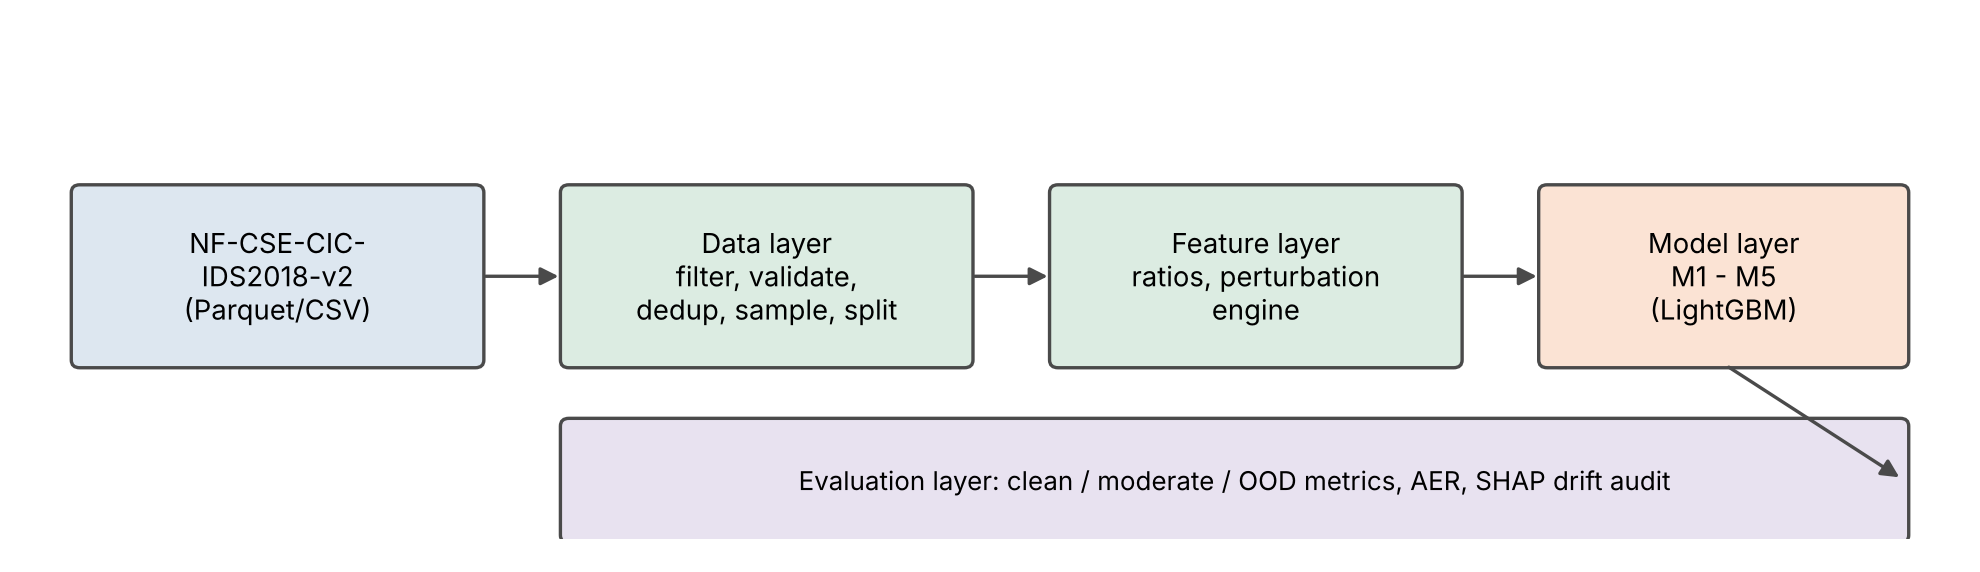
\includegraphics[width=5.8in]{assets/fig_3_1_architecture.png}
\caption{High-level system architecture: data, feature, model and evaluation layers.}
\end{figure}
The system is organised into four layers (Figure 3.1). The data layer streams the raw dataset in bounded-size chunks, filters it to the four project classes, validates every numeric field, removes exact duplicate flows, and draws a fixed, reproducible stratified sample that is split once into training and test pools. The feature layer computes the eight engineered timing-invariant ratios used by the hybrid model and implements the pacing perturbation engine. The model layer trains the five LightGBM configurations under identical hyperparameters. The evaluation layer computes clean, moderate- and out-of-distribution-perturbation metrics, the Attack Evasion Rate, and the non-circular SHAP attribution-drift audit.

\section{Threat Model}
The adversary is assumed to control the pacing of their own attack traffic --- how quickly packets within one flow are sent --- but not its structural characteristics: the destination port being targeted, the transport protocol, the TCP flags set over the flow's lifetime, the total bytes and packets transferred, or the distribution of individual packet sizes, since these are fixed by the tool or protocol the attacker is using to carry out the attack (volumetric flooding or credential brute-forcing) rather than by a choice the attacker is free to make without changing what the attack is. Benign traffic is never perturbed, since the adversary has no reason or ability to alter traffic they do not control. The adversary is evaluated under two regimes: a moderate stretch ($\alpha$ drawn independently per flow from Uniform(1.5, 2.5)) and a stronger, out-of-distribution stretch ($\alpha$ from Uniform(3.0, 4.5)), the latter never seen during any model's training.

\section{Functional Components}
\begin{table}[h]\centering
\caption{Functional components of the proposed system and the module implementing each}
\begin{tabularx}{\linewidth}{XX}
\toprule
\textbf{Component} & \textbf{Responsibility} \\
\midrule
Ingestion & Two-pass, chunked reading of the raw dataset; label mapping; schema verification \\
Validation & Finite/non-negative checks on all 40 model features; zero-duration and timer-wrap flagging \\
Deduplication & Hash-based exact-duplicate detection with conflicting-label reporting \\
Sampling and split & Largest-remainder stratified sampling; single 70/30 stratified train/test split \\
Identity checks & Empirical verification of which rate columns may be scaled under perturbation \\
Feature engineering & Eight engineered timing-invariant ratios (M5 only) \\
Perturbation engine & Consistency-preserving pacing transformation and its 9-invariant verifier \\
Model training & Shared LightGBM wrapper enforcing identical hyperparameters across M1--M5 \\
SHAP selection & Importance-share-based selection of M5's frozen feature list \\
Evaluation & Clean/moderate/OOD metrics, Attack Evasion Rate, post-perturbation recall \\
Explainability audit & Non-circular, ground-truth-class SHAP attribution-drift audit \\
\bottomrule
\end{tabularx}
\end{table}
\section{Data Flow}
\begin{figure}[h]\centering
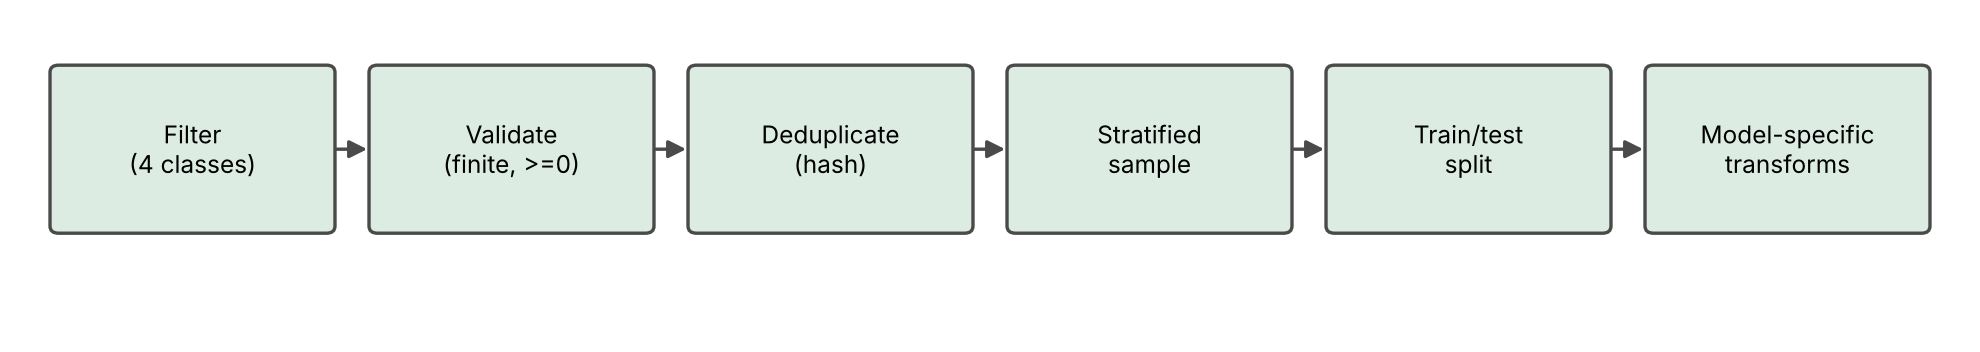
\includegraphics[width=5.8in]{assets/fig_3_2_pipeline.png}
\caption{Fixed data-processing order: filter, validate, deduplicate, sample, split, then model-specific transformations.}
\end{figure}
The order shown in Figure 3.2 is fixed and is never reordered anywhere in the implementation: nothing that depends on the test split, or on any individual model, is allowed to happen before the split itself. Deduplication happens before sampling, so that near-identical flows cannot be drawn into both the training and test pools; the stratified split happens before any feature engineering, scaling, noise injection, SHAP analysis or adversarial augmentation, so that no model-specific transformation is ever fitted on data that includes test flows.

\section{Model Progression}
\begin{figure}[h]\centering
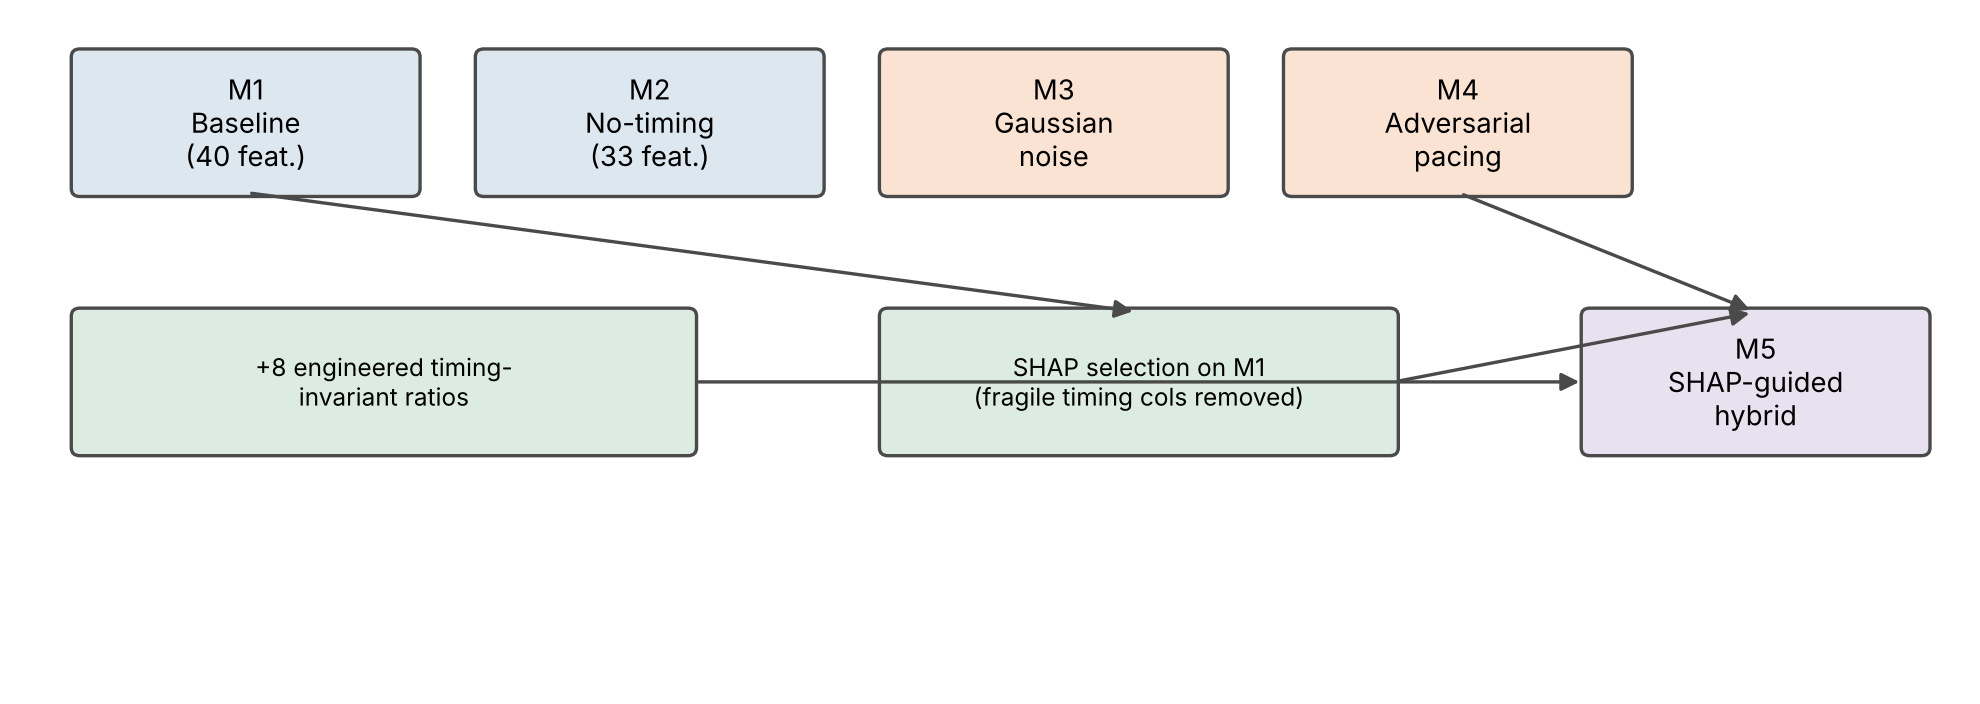
\includegraphics[width=5.8in]{assets/fig_3_3_progression.png}
\caption{The five-model progression M1--M5 and how M5's feature layer is constructed.}
\end{figure}
\begin{table}[h]\centering
\caption{The five experimental models and what each isolates}
\begin{tabularx}{\linewidth}{XXXX}
\toprule
\textbf{Model} & \textbf{Feature matrix} & \textbf{Training data} & \textbf{Question it isolates} \\
\midrule
M1 & All 40 model-input features & Clean training pool & How much does a standard baseline rely on timing features, and how evadable is it? \\
M2 & 33 structural features only & Clean training pool & Does removing all timing features solve evasion, and at what cost to clean accuracy? \\
M3 & Same 40 as M1 & Clean pool + 1 Gaussian-noise copy per training attack flow & Does unguided noise augmentation match structured hardening? \\
M4 & Same 40 as M1 & Clean pool + 1 consistency-preserving slowed copy per training attack flow & How much does structured adversarial pacing augmentation alone help? \\
M5 & 46 features: structural + SHAP-unflagged timing + 8 engineered ratios & Same augmented pool as M4 & Does SHAP-guided feature selection plus adversarial training recover M2's accuracy while improving robustness over M4? \\
\bottomrule
\end{tabularx}
\end{table}
\section{Design Rationale}
Several design choices in this system were made deliberately rather than by convention. All five models use identical LightGBM hyperparameters (class\_weight='balanced', 300 estimators, learning rate 0.1) so that any difference in their behaviour can be attributed to their feature matrix and training data, not to independent tuning that could make one model appear better than another for reasons unrelated to the research questions. The perturbation engine's rate-column scaling is gated on an empirical identity check against the real training data, rather than assumed to hold, because a perturbation that silently scales a column the data does not actually support would produce physically meaningless flows and an uninterpretable evasion result. The SHAP attribution-drift audit explains every flow for its ground-truth class, never its predicted class, and defines its audited flow set using only the baseline model's (M1's) own predictions, never M4's or M5's --- this is what makes the audit non-circular, since neither the choice of which flows to explain nor the class being explained can be influenced by the very defence being evaluated.

\begin{center}CHAPTER 4\end{center}
\begin{center}\textbf{DATASET AND METHODOLOGY}\end{center}\vspace{4pt}
\chapter{Dataset and Methodology}
\section{Dataset Description}
The project uses NF-CSE-CIC-IDS2018-v2 (Sarhan et al.), a standardized NetFlow v9 re-export of the AWS-hosted CSE-CIC-IDS2018 testbed (Sharafaldin et al., 2018), published with 43 features plus a binary Label and a 15-value Attack column. The official UQ dataset host was not reachable from the project's execution environment, so the dataset was obtained instead from a Kaggle mirror ('dhoogla/nfcsecicids2018v2'), supplied as a single Parquet file. Before use, this mirror's schema was verified programmatically against the published 43-feature definition and found identical, and all 15 original Attack label strings (including the dataset's own misspelling, 'Infilteration') were verified to match exactly, with fully consistent binary labels (0 for Benign, 1 for every attack label, with no exceptions across the full file).

Two differences from the officially published statistics were found and are reported rather than concealed. First, this mirror omits the IPV4\_SRC\_ADDR and IPV4\_DST\_ADDR columns (privacy-stripped upstream), which is harmless since both are dropped as identifiers in any case. Second, the file contains 17,129,715 rows rather than the 18,893,708 rows reported in the original publication; the DoS (483,999) and Brute-Force (120,912) class counts match the published figures exactly, while Benign and DDoS are lower, consistent with this mirror having had exact-duplicate flows already removed upstream --- a conclusion independently supported by this project's own deduplication step finding zero further conflicting-label duplicates in the file.

\section{Feature Description}
The published schema defines 43 features, of which 3 (IPV4\_SRC\_ADDR, IPV4\_DST\_ADDR, L4\_SRC\_PORT) are treated as identifiers and dropped from every model, leaving 40 model-input features: 33 structural features, which are invariant under the pacing perturbation, and 7 timing/rate features, which are the perturbation's targets. L4\_DST\_PORT is a structural feature and is never dropped. Table 4.1 lists the full structural set; Table 4.2 lists the timing/rate set.

\begin{table}[h]\centering
\caption{The 33 structural (timing-invariant) model-input features}
\begin{tabularx}{\linewidth}{XX}
\toprule
\textbf{\#} & \textbf{Feature} \\
\midrule
1 & L4\_DST\_PORT \\
2 & PROTOCOL \\
3 & L7\_PROTO \\
4 & IN\_BYTES \\
5 & OUT\_BYTES \\
6 & IN\_PKTS \\
7 & OUT\_PKTS \\
8 & TCP\_FLAGS \\
9 & CLIENT\_TCP\_FLAGS \\
10 & SERVER\_TCP\_FLAGS \\
11 & MIN\_TTL \\
12 & MAX\_TTL \\
13 & LONGEST\_FLOW\_PKT \\
14 & SHORTEST\_FLOW\_PKT \\
15 & MIN\_IP\_PKT\_LEN \\
16 & MAX\_IP\_PKT\_LEN \\
17 & RETRANSMITTED\_IN\_BYTES \\
18 & RETRANSMITTED\_IN\_PKTS \\
19 & RETRANSMITTED\_OUT\_BYTES \\
20 & RETRANSMITTED\_OUT\_PKTS \\
21 & NUM\_PKTS\_UP\_TO\_128\_BYTES \\
22 & NUM\_PKTS\_128\_TO\_256\_BYTES \\
23 & NUM\_PKTS\_256\_TO\_512\_BYTES \\
24 & NUM\_PKTS\_512\_TO\_1024\_BYTES \\
25 & NUM\_PKTS\_1024\_TO\_1514\_BYTES \\
26 & TCP\_WIN\_MAX\_IN \\
27 & TCP\_WIN\_MAX\_OUT \\
28 & ICMP\_TYPE \\
29 & ICMP\_IPV4\_TYPE \\
30 & DNS\_QUERY\_ID \\
31 & DNS\_QUERY\_TYPE \\
32 & DNS\_TTL\_ANSWER \\
33 & FTP\_COMMAND\_RET\_CODE \\
\bottomrule
\end{tabularx}
\end{table}
\begin{table}[h]\centering
\caption{The 7 timing/rate model-input features (the perturbation engine's targets)}
\begin{tabularx}{\linewidth}{XXX}
\toprule
\textbf{\#} & \textbf{Feature} & \textbf{Role under perturbation} \\
\midrule
1 & FLOW\_DURATION\_MILLISECONDS & Duration (x alpha) \\
2 & DURATION\_IN & Duration (x alpha) \\
3 & DURATION\_OUT & Duration (x alpha) \\
4 & SRC\_TO\_DST\_SECOND\_BYTES & Rate (/ alpha, if empirically approved) \\
5 & DST\_TO\_SRC\_SECOND\_BYTES & Rate (/ alpha, if empirically approved) \\
6 & SRC\_TO\_DST\_AVG\_THROUGHPUT & Rate (/ alpha, if empirically approved) \\
7 & DST\_TO\_SRC\_AVG\_THROUGHPUT & Rate (/ alpha, if empirically approved) \\
\bottomrule
\end{tabularx}
\end{table}
\section{Class Labels}
Four project classes are used, mapped from the original Attack strings by exact match only (never by substring matching, which could otherwise confuse, for example, 'Brute Force-Web' with 'FTP-BruteForce'):

\begin{table}[h]\centering
\caption{Original-label to project-class mapping (Appendix B of the project proposal)}
\begin{tabularx}{\linewidth}{XX}
\toprule
\textbf{Project class} & \textbf{Original Attack labels} \\
\midrule
Benign & Benign \\
DDoS & DDOS attack-HOIC; DDOS attack-LOIC-UDP; DDoS attacks-LOIC-HTTP \\
DoS & DoS attacks-GoldenEye; DoS attacks-Hulk; DoS attacks-SlowHTTPTest; DoS attacks-Slowloris \\
Brute-Force & FTP-BruteForce; SSH-Bruteforce \\
\bottomrule
\end{tabularx}
\end{table}
Bot, Infilteration (the dataset's own spelling) and the three web-application attacks are excluded by design: they are out of scope for a pacing-based threat model, not excluded for rarity. Any Attack label encountered that is not one of these 15 strings halts the pipeline rather than being silently mapped; none were encountered in the real file.

\section{Data Preprocessing}
The raw file is read in two passes to remain memory-safe on a dataset of this size. Pass 1 streams the file in chunks of 200,000 rows, filters each chunk to the four project classes, validates and hashes every valid row, and retains only a compact record (hash, class, row position) rather than the row itself. Pass 2 re-reads the file and extracts only the globally selected rows that will form the final 100,000-flow sample. On the real file, Pass 1 scanned 17,129,715 rows in approximately 1 minute 43 seconds and found 16,982,667 eligible across the four classes.

\section{Data Validation}
Every one of the 40 model features is checked, for every valid row, to be numeric, finite and non-negative; a row failing any check is dropped and counted by reason, never silently discarded. On the real dataset, zero rows failed any validation check across the full 16,982,667 eligible rows. Validation also flags (without altering) zero-duration flows and near-32-bit-timer-wrap anomalies, reported separately per duration column. This surfaced a genuine, previously undocumented data-quality finding: FLOW\_DURATION\_MILLISECONDS is 0 for 86.1\% of valid flows, and 99.1\% of its remaining non-zero values cluster within 1,000 ms of 2$^3$$^2$ microseconds ($\approx$ 4,294,967.296 ms) --- a signature of a 32-bit microsecond counter overflow in the nProbe NetFlow exporter used to build this dataset. DURATION\_IN and DURATION\_OUT do not show this pattern and were confirmed, independently of this project's own code, to have sane distributions (maxima of the order of 10$^4$--5 ms).

\section{Duplicate Handling}
The duplicate key is a 64-bit hash of the 40 model-input feature values together with the project class label, computed over a canonical byte representation so that identical feature values always hash identically. Where two rows share features but carry conflicting labels, one copy of each distinct (features, label) pair is retained and every such conflict is logged rather than being silently resolved; on the real data, zero conflicting-label groups were found. After deduplication, the unique eligible counts per class were: Benign 8,488,924; DDoS 114,638; DoS 338,755; Brute-Force 14,720.

\section{Sampling}
A 100,000-flow sample is drawn with per-class quotas computed by the largest-remainder method (quota\_c = 100,000 $\times$ unique\_c / total\_unique, rounded down, with the remaining units given to the classes with the largest fractional remainder, so quotas sum to exactly 100,000 without artificially rebalancing the classes), then sampled uniformly without replacement within each class using a fixed seed (42). The resulting quotas, computed from the real post-deduplication counts, are shown in Table 4.5.

\begin{table}[h]\centering
\caption{Largest-remainder sampling quotas, computed from the real post-deduplication class counts}
\begin{tabularx}{\linewidth}{XXXX}
\toprule
\textbf{Project class} & \textbf{Unique eligible rows} & \textbf{Share of unique} & \textbf{Quota} \\
\midrule
Benign & 8,488,924 & 94.77\% & 94,774 \\
DDoS & 114,638 & 1.28\% & 1,280 \\
DoS & 338,755 & 3.78\% & 3,782 \\
Brute-Force & 14,720 & 0.16\% & 164 \\
Total & 8,957,037 & 100.00\% & 100,000 \\
\bottomrule
\end{tabularx}
\end{table}
\section{Train-Test Split}
The 100,000-flow sample is split once into a 70\% training pool (70,000 flows) and a 30\% test pool (30,000 flows) by stratified sampling on the project class, using a fixed seed (42). This split is performed before any feature engineering, scaling, noise injection, SHAP analysis or adversarial augmentation, and is reused unchanged by every one of the five models and every one of the five experimental seeds, so that no model ever sees a different split and no comparison between models can be attributed to a difference in data.

\section{Feature Engineering}
The SHAP-guided hybrid model (M5) uses eight engineered ratios that are mathematically guaranteed invariant under the pacing perturbation, because every quantity they are computed from (bytes and packet counts) is itself held fixed:

\begin{itemize}\setlength\itemsep{2pt}\item BPP\_IN = IN\_BYTES / max(IN\_PKTS, 1)\end{itemize}
\begin{itemize}\setlength\itemsep{2pt}\item BPP\_OUT = OUT\_BYTES / max(OUT\_PKTS, 1)\end{itemize}
\begin{itemize}\setlength\itemsep{2pt}\item DIR\_RATIO = IN\_BYTES / (OUT\_BYTES + 1)\end{itemize}
\begin{itemize}\setlength\itemsep{2pt}\item SHARE\_128, SHARE\_128\_256, SHARE\_256\_512, SHARE\_512\_1024, SHARE\_1024\_1514 = the corresponding NUM\_PKTS\_* bin divided by the packet-count denominator\end{itemize}
The packet-size-bin denominator was not assumed but checked empirically against the real data: the five NUM\_PKTS\_* bins were found to sum to IN\_PKTS + OUT\_PKTS in 93.5\% of flows, rather than to IN\_PKTS alone (only a 3.7\% match rate), so max(IN\_PKTS + OUT\_PKTS, 1) is used as the denominator for all five share features.

\section{Adversarial Perturbation}
\begin{figure}[h]\centering
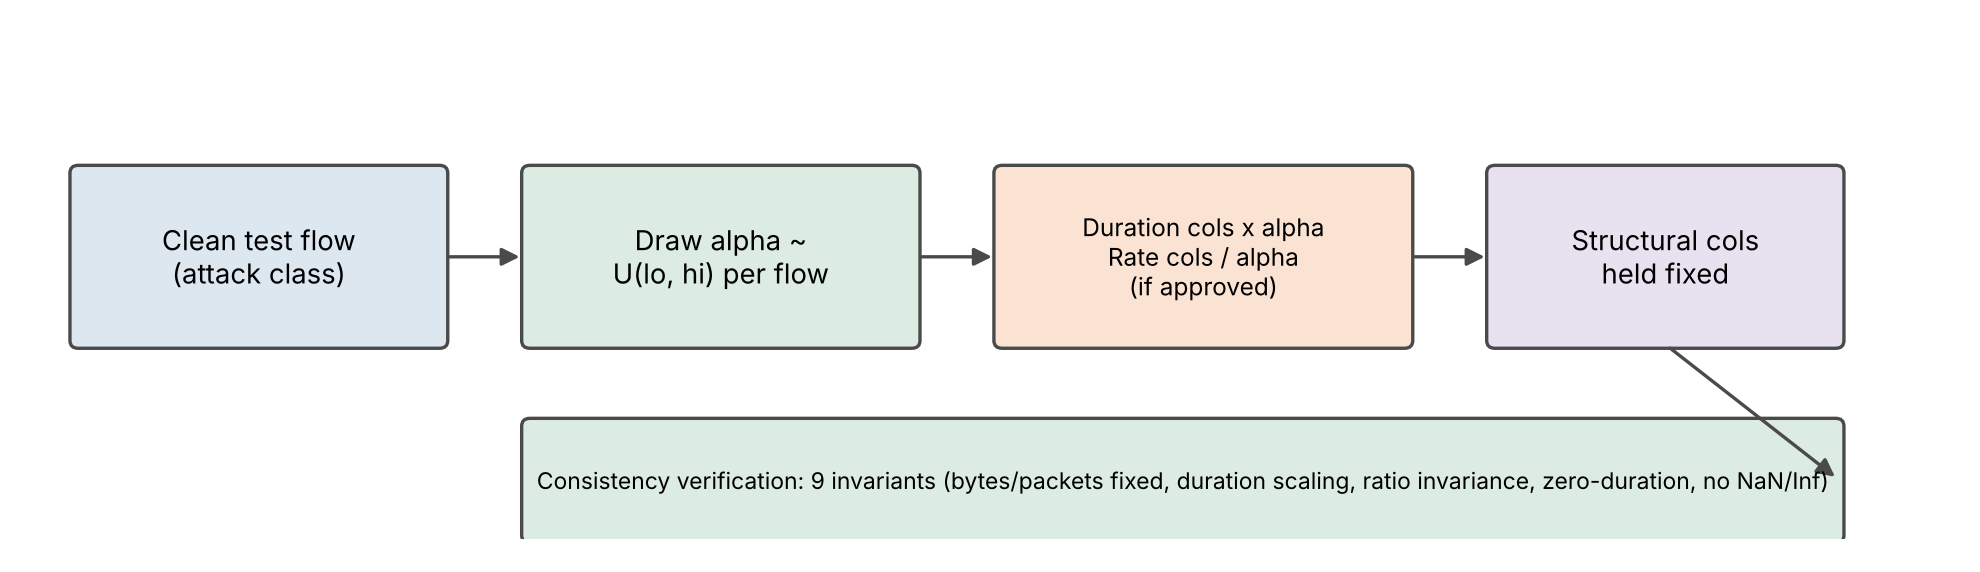
\includegraphics[width=5.8in]{assets/fig_4_1_perturbation.png}
\caption{The consistency-preserving pacing perturbation workflow and its verification step.}
\end{figure}
For every attack flow in the test (or, for augmentation, training) pool, an independent stretch factor is drawn: alpha \textasciitilde{} Uniform(1.5, 2.5) for the moderate regime and the training-augmentation regime, and alpha \textasciitilde{} Uniform(3.0, 4.5) for the out-of-distribution regime, which is never seen during training by any model. The three duration features are multiplied by alpha; a zero-duration flow is therefore left unchanged by construction (0 $\times$ alpha = 0). The four rate/throughput features are divided by alpha only if Phase 1's empirical identity check approves that specific column for this treatment; every other model feature --- all 33 structural features --- is left exactly unchanged. Benign flows are never perturbed.

The identity check that gates rate-column scaling tests, for each rate column, every plausible bytes/duration relationship (both candidate duration columns, both bytes/second and bits/second unit conventions) against the real training data, and approves a column only if its best candidate holds within 5\% relative error for at least 95\% of positive-duration flows. On the real data, none of the four rate/throughput columns met this bar (the best candidate for any of them held for at most 29.4\% of flows), so all four were held fixed under every perturbation applied in this project --- a genuine empirical finding, not a design assumption, and documented in full in Chapter 6.

After perturbation, nine algebraic invariants are verified automatically: every structural feature is checked to be byte-identical before and after; durations are checked to scale by exactly alpha; rate columns are checked to scale by exactly 1/alpha if approved, or to remain exactly fixed if not; the rate$\times$duration product is checked to remain constant for any approved rate column; the eight engineered ratios are checked to be unchanged; Benign rows are checked to be completely untouched; zero-duration flows are checked to remain zero; no NaN or Inf value is checked to have been introduced; and every drawn alpha is checked to be at least 1.0 for an attack flow. All 450 such checks (45 invariants $\times$ 5 seeds $\times$ 2 regimes) passed on the real data.

\section{Model Training}
All five models use LGBMClassifier(class\_weight='balanced') with identical hyperparameters: n\_estimators=300, learning\_rate=0.1, num\_leaves=31, subsample=0.8, subsample\_freq=1, colsample\_bytree=0.8. Only the feature matrix, the training data, and the random seed differ between models, enforced in code by a single shared training function that every model is built through. M3 and M4 each add exactly one synthetic copy of every training attack flow (verified to double the attack portion of the training pool exactly) --- a Gaussian-noise copy for M3 (with sigma = 0.10 times each continuous feature's own training standard deviation, clipped at zero, and excluding discrete fields such as ports, flags, TTLs and protocol codes) and a consistency-preserving slowed copy for M4 and M5.

\section{Experimental Design}
\begin{figure}[h]\centering
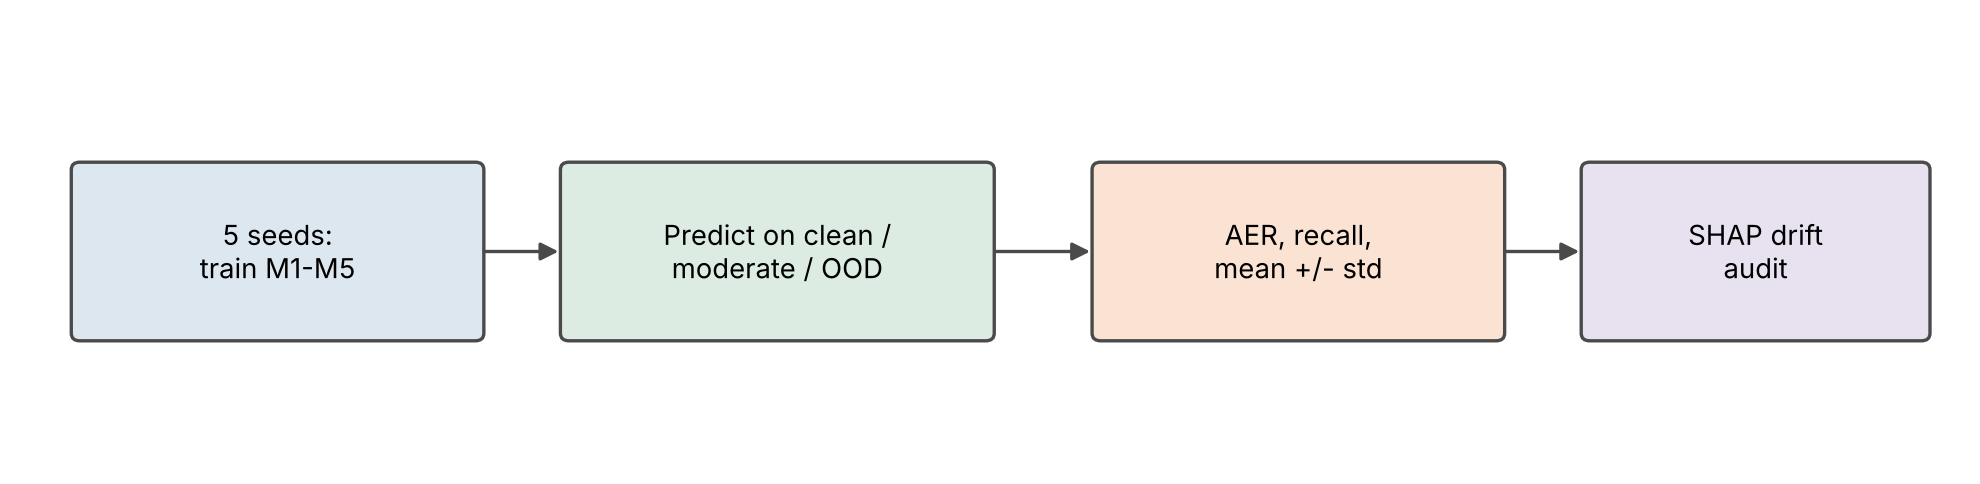
\includegraphics[width=5.8in]{assets/fig_4_4_eval_workflow.png}
\caption{The full 5-seed experimental evaluation workflow.}
\end{figure}
Every model is retrained independently at five fixed seeds (42, 101, 202, 303, 404), re-drawing the Gaussian noise or the adversarial slowing for that seed, while the underlying 100,000-flow sample and its 70/30 split are never re-drawn. Each trained model is evaluated on the clean test set and on that seed's moderate and out-of-distribution perturbed test sets. Results are reported as mean $\pm$ sample standard deviation over n = 5 seeds, which measures variability from model training and perturbation randomness conditional on one fixed sample and split, not variability from re-sampling or re-splitting the data.

\section{Evaluation Metrics}
The following metrics are computed for every model, at every seed:

\begin{itemize}\setlength\itemsep{2pt}\item Per-class precision, recall and F1-score, plus macro-F1 and weighted-F1, on the clean test set.\end{itemize}
\begin{itemize}\setlength\itemsep{2pt}\item Clean False Positive Rate (FPR): the share of Benign test flows predicted as any attack class (Benign flows are never perturbed, so this always measures clean behaviour).\end{itemize}
\begin{itemize}\setlength\itemsep{2pt}\item Binary attack-detection recall: the share of attack test flows predicted as non-Benign.\end{itemize}
\begin{itemize}\setlength\itemsep{2pt}\item Attack Evasion Rate (AER): for model m, let D\_m be the attack flows the clean test set that m correctly flags as non-Benign. AER\_m = (flows in D\_m predicted Benign after perturbation) / |D\_m| x 100\%. Reclassification into a different attack class is not counted as evasion --- only a post-perturbation prediction of Benign is.\end{itemize}
\begin{itemize}\setlength\itemsep{2pt}\item Post-perturbation attack recall: computed over the entire perturbed attack test set, not only D\_m, so that attacks already missed on clean data are also represented.\end{itemize}
AER is computed overall and separately for DDoS, DoS and Brute-Force, with the denominator count reported alongside every value and classes with fewer than 200 supporting flows explicitly flagged as low-support, since Brute-Force in particular is expected to contribute only a small number of test flows.

\begin{center}CHAPTER 5\end{center}
\begin{center}\textbf{IMPLEMENTATION}\end{center}\vspace{4pt}
\chapter{Implementation}
\section{Programming Languages}
The entire system is implemented in Python 3.13. Python was chosen for its mature data-science ecosystem (pandas, NumPy, scikit-learn), its first-class LightGBM and SHAP bindings, and because it allows the data pipeline, the model training code and the evaluation and reporting code to share a single, typed codebase with no language boundary to maintain.

\section{Libraries and Frameworks}
\begin{table}[h]\centering
\caption{Core libraries used, with the version actually installed and verified}
\begin{tabularx}{\linewidth}{XXX}
\toprule
\textbf{Library} & \textbf{Version} & \textbf{Purpose} \\
\midrule
pandas & 3.1.1 & Tabular data handling, chunked CSV/Parquet ingestion \\
NumPy & 2.5.5 & Vectorised numerical computation, random number generation \\
PyArrow & 26.0.1 & Parquet reading/writing, chunked Parquet streaming \\
scikit-learn & 1.9.1 & Stratified train/test split, evaluation metrics \\
LightGBM & 4.7.0 & Gradient-boosted decision tree classifier (all 5 models) \\
SHAP & 0.54.1 & TreeExplainer-based Shapley-value attribution \\
Matplotlib & 3.11.2 & Comparison charts, SHAP summary and waterfall plots \\
Pydantic & 2.14.4 & Validated experiment configuration loading \\
pytest & 9.2.0 & Automated unit and integration testing \\
\bottomrule
\end{tabularx}
\end{table}
\section{Development Environment}
Development and all experiments were carried out in a cloud Linux container (Python 3.13, 4 CPU cores, 15 GB RAM) with no GPU, confirming that the entire pipeline --- including training all five LightGBM models across five seeds on the 100,000-flow sample --- runs comfortably on free, CPU-only compute, as the original project proposal required. Version control was managed with Git, with each phase of the pipeline (data ingestion, baseline models, perturbation engine, robustness models, full evaluation, reporting) committed and pushed separately.

\section{Project Structure}
The codebase follows a modular package layout, so that each pipeline stage is independently testable:

\begin{itemize}\setlength\itemsep{2pt}\item src/nids/config --- Pydantic-validated loading of configs/experiment.yaml, the single file defining every experimental parameter.\end{itemize}
\begin{itemize}\setlength\itemsep{2pt}\item src/nids/data --- ingestion, label mapping, validation, deduplication, sampling, splitting, schema and rate/duration identity checks.\end{itemize}
\begin{itemize}\setlength\itemsep{2pt}\item src/nids/features --- the canonical feature-group definitions and the engineered-ratio computation.\end{itemize}
\begin{itemize}\setlength\itemsep{2pt}\item src/nids/perturbation --- the pacing perturbation engine and its consistency verifier.\end{itemize}
\begin{itemize}\setlength\itemsep{2pt}\item src/nids/models --- the shared LightGBM training wrapper, M3/M4 augmentation, and M5's SHAP-based feature selection.\end{itemize}
\begin{itemize}\setlength\itemsep{2pt}\item src/nids/evaluation --- clean/attack-evasion metrics and 5-seed mean$\pm$std aggregation.\end{itemize}
\begin{itemize}\setlength\itemsep{2pt}\item src/nids/explainability --- the non-circular SHAP attribution-drift audit.\end{itemize}
\begin{itemize}\setlength\itemsep{2pt}\item scripts/ --- one driver script per phase (run\_pipeline.py, run\_phase2.py ... run\_phase5.py, generate\_report.py), each idempotent and resuming from the previous phase's saved artifacts.\end{itemize}
\begin{itemize}\setlength\itemsep{2pt}\item tests/ --- 94 automated pytest tests, all run against small synthetic NetFlow-shaped fixtures so the full 17-million-row dataset is never required to verify correctness.\end{itemize}
\section{Data Processing Pipeline}
scripts/run\_pipeline.py implements the two-pass ingestion described in Section 4.4. It supports both CSV and Parquet input transparently, detecting the format from the file extension; Parquet is read through pyarrow.ParquetFile.iter\_batches, which decodes a file incrementally in bounded-size batches even when, as with the real dataset obtained for this project, the entire file is stored as a single Parquet row group. Every stage of the pipeline (schema verification, label mapping, validation, deduplication, sampling, splitting) writes a corresponding report file to disk, so that the pipeline's behaviour on the real data is fully auditable after the fact rather than only visible in console output.

\section{LightGBM Model Implementation}
A single function, fit\_model(), builds every one of the five models: it asserts that the requested feature list contains no target or identifier column (a leakage guard that raises an error rather than silently training on a label column), constructs an LGBMClassifier with the project's fixed hyperparameters and the requested seed, and fits it. Because every model is built through this one function, it is structurally impossible for two models in this project to differ by hyperparameter alone.

\section{Adversarial Sample Generation}
The perturbation engine (src/nids/perturbation/pacing.py) draws one alpha per attack flow with NumPy's modern Generator API seeded per experimental seed, applies the duration and (where approved) rate transformations described in Section 4.10 using vectorised array operations rather than a per-row Python loop, and recomputes the engineered ratio columns afterwards for correctness even though, on this dataset, their inputs are never altered by the perturbation. The training-time augmentation functions (gaussian\_noise\_augment and adversarial\_pacing\_augment) reuse this same perturbation machinery, so the M4 training-time transformation and the evaluation-time attack are, by construction, the identical code path.

One real implementation defect was found and fixed during this work: a pathological outlier in SRC\_TO\_DST\_SECOND\_BYTES (a single flow with a value of approximately 8.9 $\times$ 10$^2$$^0$$^1$, consistent with the exporter's known rate-column corruption) made the naive standard-deviation computation underlying the Gaussian-noise augmenter overflow to infinity, which would have injected unbounded noise into every row of that column. The augmenter now treats a non-finite standard deviation the same way it treats a genuinely zero-variance column --- by leaving that column fixed --- and a regression test was added to guard against the defect recurring.

\section{SHAP Analysis}
SHAP values are computed with shap.TreeExplainer in raw-margin (log-odds) output space, never on test data. For M5's feature-selection step, a class-capped subset of at most 2,500 training flows per class (seed 42) is explained against the trained M1 model; each timing/rate feature's importance share is its mean absolute Shapley value divided by the sum of all features' mean absolute Shapley values, averaged over the four classes, and a feature is flagged fragile if this share is at least 1/40 = 0.025. For the forensic drift audit, the same TreeExplainer machinery explains each audited flow twice --- its clean version and its out-of-distribution-perturbed version --- always for that flow's ground-truth class, for M1, M4 and M5 in turn.

\section{Hybrid Defence Implementation}
\begin{figure}[h]\centering
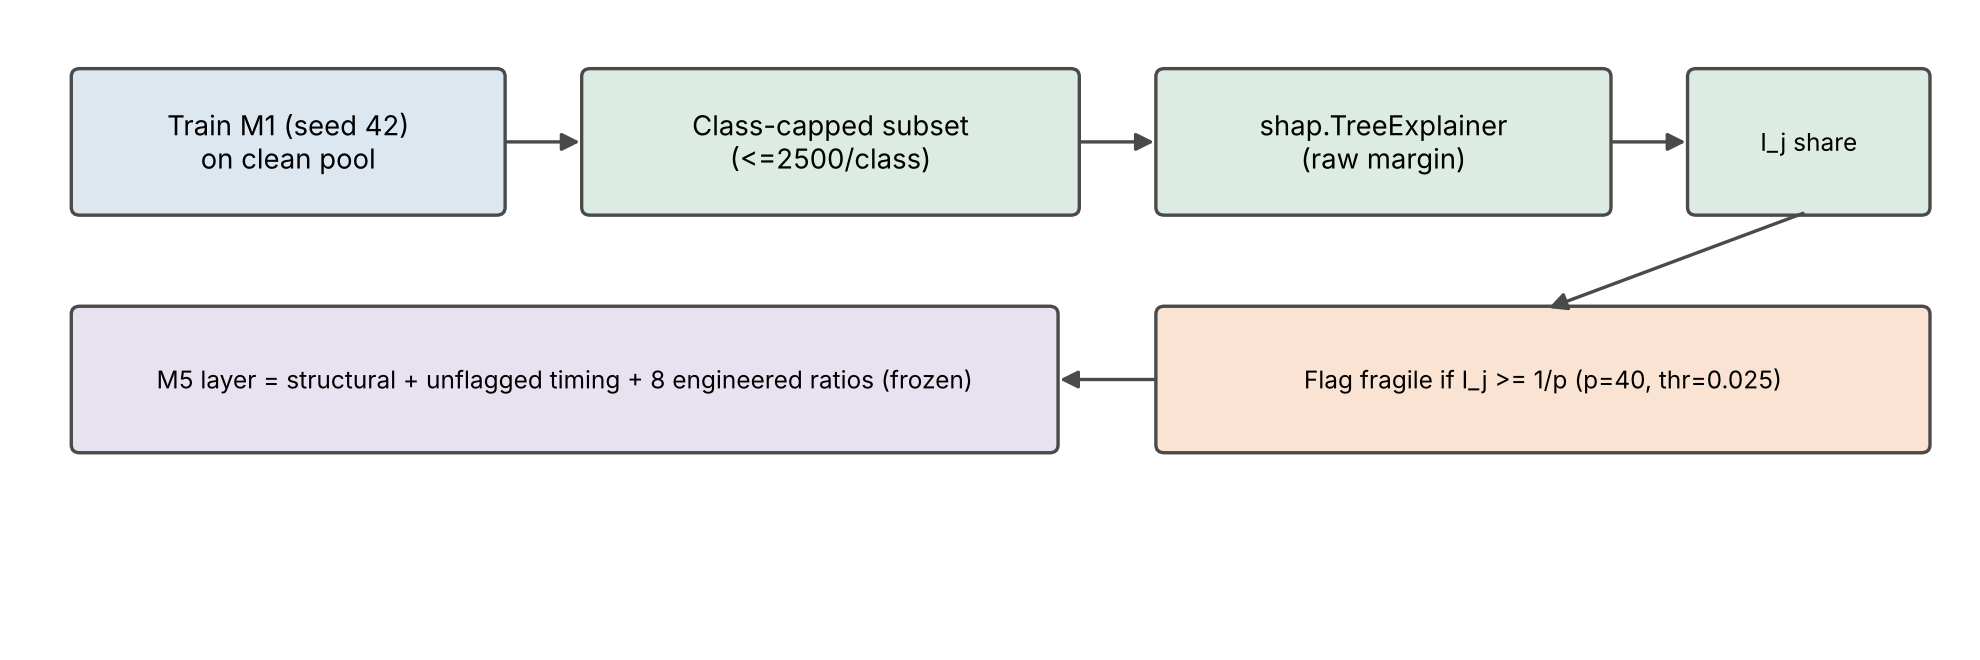
\includegraphics[width=5.8in]{assets/fig_4_2_shap_selection.png}
\caption{M5's SHAP-guided feature-selection procedure.}
\end{figure}
\begin{figure}[h]\centering
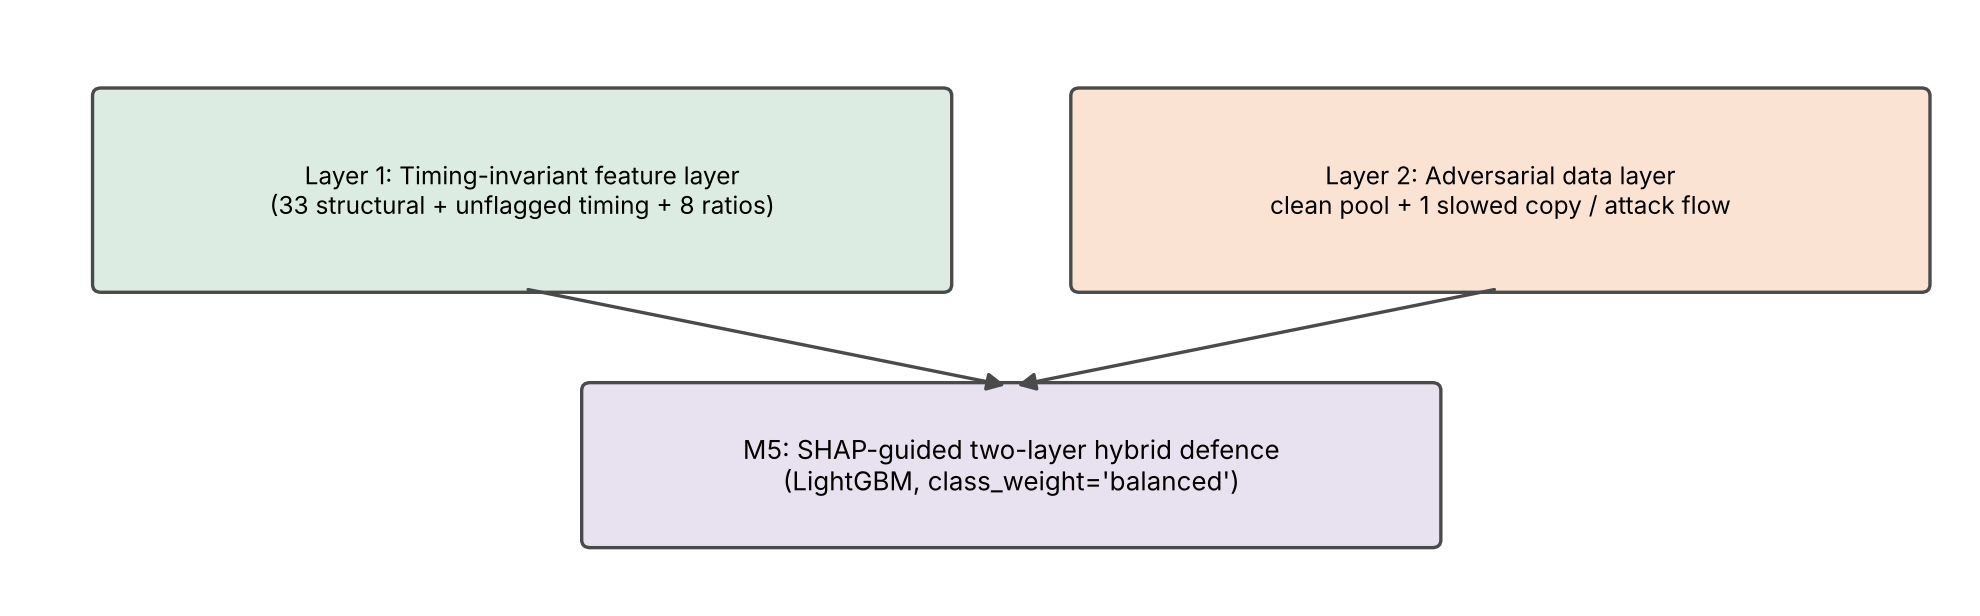
\includegraphics[width=5.8in]{assets/fig_4_3_m5_hybrid.png}
\caption{M5's two-layer hybrid architecture: a timing-invariant feature layer and an adversarially augmented data layer.}
\end{figure}
M5 is constructed in two layers. Layer 1 fixes the feature matrix: all 33 structural features, the timing/rate features SHAP did not flag as fragile, and the 8 engineered timing-invariant ratios, frozen once (at seed 42) and reused unchanged for every one of the five experimental seeds, exactly as the project proposal specifies. Layer 2 trains this feature matrix on the same adversarially augmented pool used for M4 --- the clean training rows plus one consistency-preserving slowed copy of every training attack flow --- with the eight engineered ratios recomputed for the slowed copies.

\section{Model Evaluation}
scripts/run\_phase5.py retrains all five models at each of the five seeds, generates that seed's moderate and out-of-distribution perturbed test sets, and computes every metric in Section 4.13 for every model at every seed, aggregating to mean $\pm$ standard deviation with src/nids/evaluation/aggregation.py. The same script runs the non-circular SHAP drift audit once, at seed 42, in the out-of-distribution regime, as the project proposal specifies.

\section{Output Files and Visualizations}
Every phase script writes its outputs under a single artifacts/ directory: validation and deduplication reports, the sampled and split Parquet files, the trained LightGBM model files (one per model per seed, 25 in total), clean/moderate/out-of-distribution metrics tables, confusion matrices, the Attack-Evasion-Rate table, the SHAP selection and drift-audit tables, comparison charts, and a final results\_summary.md assembled automatically from these files by scripts/generate\_report.py, so that every number quoted in Chapter 6 of this thesis traces back to a file produced by a real, logged execution rather than being typed in by hand.

\begin{center}CHAPTER 6\end{center}
\begin{center}\textbf{RESULTS AND ANALYSIS}\end{center}\vspace{4pt}
\chapter{Results and Analysis}
Every number in this chapter is read from a file produced by running the implemented pipeline on the real, 17,129,715-row NF-CSE-CIC-IDS2018-v2 dataset (see Chapter 4 and Chapter 5); none is estimated, assumed or fabricated. All models were trained and evaluated across five fixed seeds (42, 101, 202, 303, 404) on the same 70,000-flow training pool and 30,000-flow test pool.

\section{Clean Data Performance}
\begin{table}[h]\centering
\caption{Clean-test performance by model, mean $\pm$ sample standard deviation over 5 seeds}
\begin{tabularx}{\linewidth}{XXXXX}
\toprule
\textbf{Model} & \textbf{Macro-F1} & \textbf{Weighted-F1} & \textbf{Clean FPR} & \textbf{Attack recall} \\
\midrule
M1 (Baseline) & 0.9994 $\pm$ 0.0011 & 0.99996 $\pm$ 0.00002 & 0.000007 $\pm$ 0.000016 & 0.9994 $\pm$ 0.0000 \\
M2 (No-timing) & 0.9985 $\pm$ 0.0009 & 0.99987 $\pm$ 0.00008 & 0.000070 $\pm$ 0.000050 & 0.9989 $\pm$ 0.0007 \\
M3 (Gaussian noise) & 0.9999 $\pm$ 0.0000 & 0.99997 $\pm$ 0.00000 & 0.000000 $\pm$ 0.000000 & 0.9994 $\pm$ 0.0000 \\
M4 (Adversarial) & 0.9999 $\pm$ 0.0000 & 0.99997 $\pm$ 0.00000 & 0.000000 $\pm$ 0.000000 & 0.9994 $\pm$ 0.0000 \\
M5 (SHAP hybrid) & 0.9998 $\pm$ 0.0001 & 0.99995 $\pm$ 0.00002 & 0.000021 $\pm$ 0.000019 & 0.9994 $\pm$ 0.0000 \\
\bottomrule
\end{tabularx}
\end{table}
All five models reach near-ceiling clean performance. M2, which uses only the 33 structural features and no timing information at all, trails M1 by only 0.0009 macro-F1 --- a negligible cost for completely removing timing-feature reliance, and a first indication (confirmed in Section 6.9) that this dataset's four classes are heavily separable by non-timing signatures alone. M3 and M4 reach identical macro-F1 (0.9999) to four decimal places at every one of the five seeds; this was verified not to be an artefact of shared random state (each seed draws independent noise or slowing and trains an independently seeded model) but a genuine consequence of how separable this four-class problem is --- the same small number of boundary flows are resolved identically regardless of the minor randomness introduced by bagging, column sub-sampling or the augmentation itself.

\begin{table}[h]\centering
\caption{M1 per-class clean performance at seed 42 (confusion matrix in Table 6.3)}
\begin{tabularx}{\linewidth}{XXXXXX}
\toprule
\textbf{Class} & \textbf{Precision} & \textbf{Recall} & \textbf{F1-score} & \textbf{Support} & \textbf{Low support} \\
\midrule
Benign & 0.999965 & 0.999965 & 0.999965 & 28,432 & No \\
DDoS & 1.000000 & 1.000000 & 1.000000 & 384 & No \\
DoS & 1.000000 & 0.999119 & 0.999559 & 1,135 & No \\
Brute-Force & 0.980000 & 1.000000 & 0.989899 & 49 & Yes \\
Macro average & --- & --- & 0.997356 & 30,000 & --- \\
Weighted average & --- & --- & 0.999933 & 30,000 & --- \\
\bottomrule
\end{tabularx}
\end{table}
Brute-Force is flagged low-support (fewer than 200 test flows, as anticipated by the project proposal) because this already-deduplicated dataset mirror has far fewer unique Brute-Force flows than the officially published, non-deduplicated statistics would suggest; its per-class metrics are reported here, but should be read with this small sample size in mind.

\section{Adversarial Robustness}
The perturbation engine's own consistency verification passed all 450 checks (45 invariants $\times$ 5 seeds $\times$ 2 regimes), confirming that the zero-evasion result reported below reflects genuine model behaviour under a correctly implemented perturbation, not a broken or ineffective attack. The headline result, however, is a null one: the Attack Evasion Rate (AER) was 0.00\% for every model, every attack class, both the moderate and out-of-distribution regimes, and all five seeds.

\begin{table}[h]\centering
\caption{Overall Attack Evasion Rate and post-perturbation recall, mean $\pm$ std over 5 seeds}
\begin{tabularx}{\linewidth}{XXXX}
\toprule
\textbf{Model} & \textbf{Moderate AER} & \textbf{OOD AER} & \textbf{OOD post-perturbation recall} \\
\midrule
M1 & 0.00\% $\pm$ 0.00\% & 0.00\% $\pm$ 0.00\% & 0.9994 $\pm$ 0.0000 \\
M2 & 0.00\% $\pm$ 0.00\% & 0.00\% $\pm$ 0.00\% & 0.9989 $\pm$ 0.0007 \\
M3 & 0.00\% $\pm$ 0.00\% & 0.00\% $\pm$ 0.00\% & 0.9994 $\pm$ 0.0000 \\
M4 & 0.00\% $\pm$ 0.00\% & 0.00\% $\pm$ 0.00\% & 0.9994 $\pm$ 0.0000 \\
M5 & 0.00\% $\pm$ 0.00\% & 0.00\% $\pm$ 0.00\% & 0.9994 $\pm$ 0.0000 \\
\bottomrule
\end{tabularx}
\end{table}
\begin{figure}[h]\centering
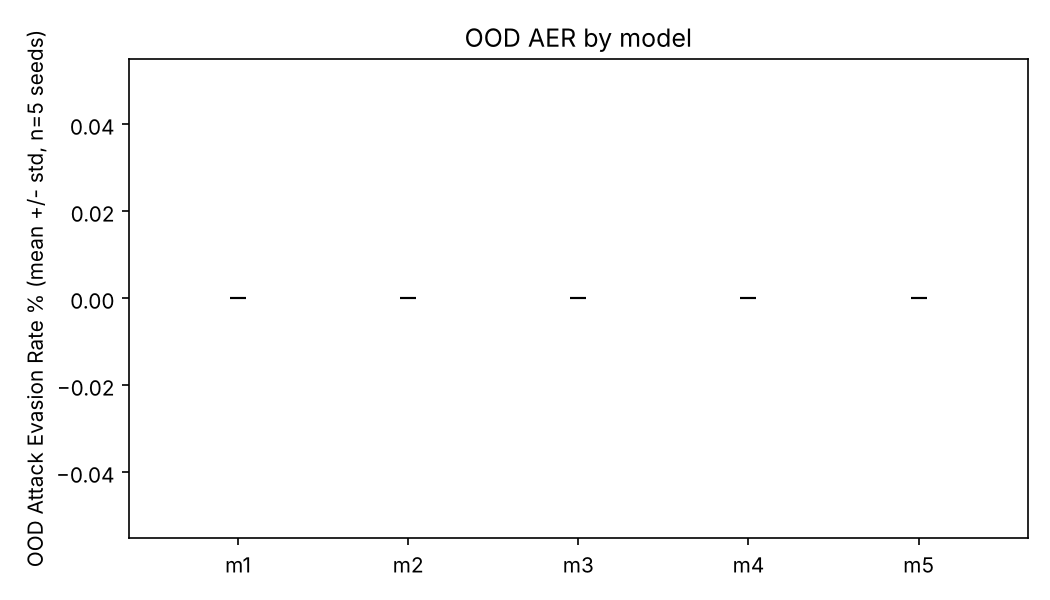
\includegraphics[width=5.8in]{assets/fig_result_aer.png}
\caption{Out-of-distribution Attack Evasion Rate by model (mean $\pm$ std over 5 seeds). All five models reach 0.00\%.}
\end{figure}
This null result is attributable to two genuine, empirically discovered properties of the dataset, not to a defect in the perturbation engine. First, none of the four rate/throughput features passed the project's own consistency-scaling check (Section 4.10): the best candidate relationship held for at most 29.4\% of flows, far short of the 95\% acceptance bar, so all four columns were held fixed and only the three duration columns could be stretched. Second, the four project classes are separable almost entirely by structural, non-timing features --- destination port, protocol, packet-size extremes and TTLs, none of which the perturbation touches --- as M2's near-identical clean performance (Section 6.1) already demonstrates directly. This is reported as a limitation of the dataset and of this specific experimental setup, not concealed or reframed as a success of the defences evaluated.

\section{Model Comparison}
\begin{figure}[h]\centering
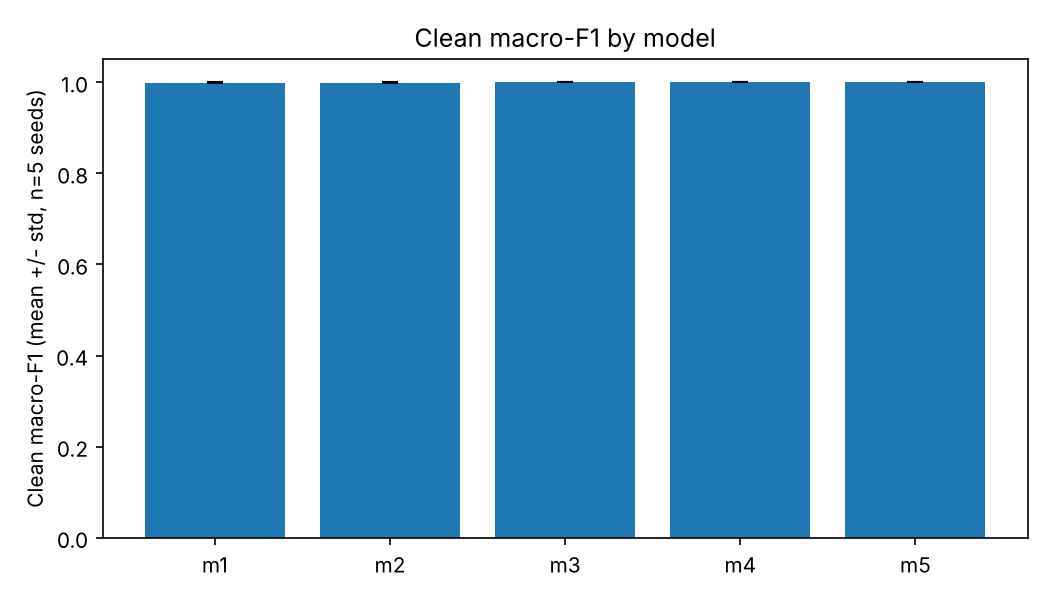
\includegraphics[width=5.8in]{assets/fig_result_macro_f1.png}
\caption{Clean macro-F1 by model (mean $\pm$ std over 5 seeds).}
\end{figure}
On clean data, M3 and M4 are the strongest (macro-F1 0.9999), M1 and M5 close behind (0.9994 and 0.9998 respectively), and M2 the weakest though still above 0.998. Because the AER comparison in Section 6.2 is uninformative here (every model reaches the same floor of 0.00\%), the SHAP attribution-drift audit in Section 6.9 is the more discriminating comparison between M1, M4 and M5 for this dataset.

\section{Per-Class Performance}
Across all five models, DDoS and DoS are detected essentially perfectly (F1 within rounding of 1.000); Brute-Force, despite its small support, is also detected with F1 above 0.98 for every model. Benign precision and recall both exceed 0.9999 for every model, so the clean false-positive rate (Section 6.5) is extremely low throughout.

\section{Confusion Matrices}
\begin{table}[h]\centering
\caption{M1 clean-test confusion matrix, seed 42 (rows: true class, columns: predicted class)}
\begin{tabularx}{\linewidth}{XXXXX}
\toprule
\textbf{True \textbackslash{} Pred} & \textbf{Benign} & \textbf{DDoS} & \textbf{DoS} & \textbf{Brute-Force} \\
\midrule
Benign & 28,431 & 0 & 0 & 1 \\
DDoS & 0 & 384 & 0 & 0 \\
DoS & 1 & 0 & 1,134 & 0 \\
Brute-Force & 0 & 0 & 0 & 49 \\
\bottomrule
\end{tabularx}
\end{table}
\begin{table}[h]\centering
\caption{M5 clean-test confusion matrix, seed 42 (rows: true class, columns: predicted class)}
\begin{tabularx}{\linewidth}{XXXXX}
\toprule
\textbf{True \textbackslash{} Pred} & \textbf{Benign} & \textbf{DDoS} & \textbf{DoS} & \textbf{Brute-Force} \\
\midrule
Benign & 28,432 & 0 & 0 & 0 \\
DDoS & 0 & 384 & 0 & 0 \\
DoS & 1 & 0 & 1,134 & 0 \\
Brute-Force & 0 & 0 & 0 & 49 \\
\bottomrule
\end{tabularx}
\end{table}
M5 makes one fewer error than M1 at seed 42 (zero Benign flows misclassified, versus one for M1), consistent with M5's marginally higher weighted-F1 observed in Table 6.1, although both models' error counts are too small (1--2 flows out of 30,000) to draw a statistically strong conclusion from a single seed.

\section{Precision, Recall, and F1-Score}
Precision, recall and F1-score for every class and every model, at every seed, are reported in full in the project's artifacts/metrics/ directory (clean\_metrics\_per\_class.csv, metrics\_moderate.csv, metrics\_ood.csv); the headline macro- and weighted-F1 values are summarised in Table 6.1 above. No model's moderate- or out-of-distribution-perturbation per-class metrics differ meaningfully from its clean metrics, which is the per-class expression of the overall 0.00\% AER result in Section 6.2.

\section{False Positive Rate}
Since Benign test flows are never perturbed (Section 4.10), the clean False Positive Rate reported in Table 6.1 is identical under every perturbation regime for every model. All five models keep the clean FPR below 0.0001 (one false alarm in ten thousand benign flows or fewer); M3 and M4 reach exactly zero false positives across every seed.

\section{Attack Evasion Rate}
Attack Evasion Rate is reported in full, by class, in Table 6.2 and in the project's aer\_by\_class.csv; every per-class value, for every model, every regime and every seed, is 0.00\%. The denominator counts behind this figure (the number of attack flows each model correctly detects on clean data, before perturbation) are reported alongside every AER value, per the project's own low-support policy, and are never below 49 flows (Brute-Force) for any model or seed.

\section{SHAP Analysis}
\begin{figure}[h]\centering
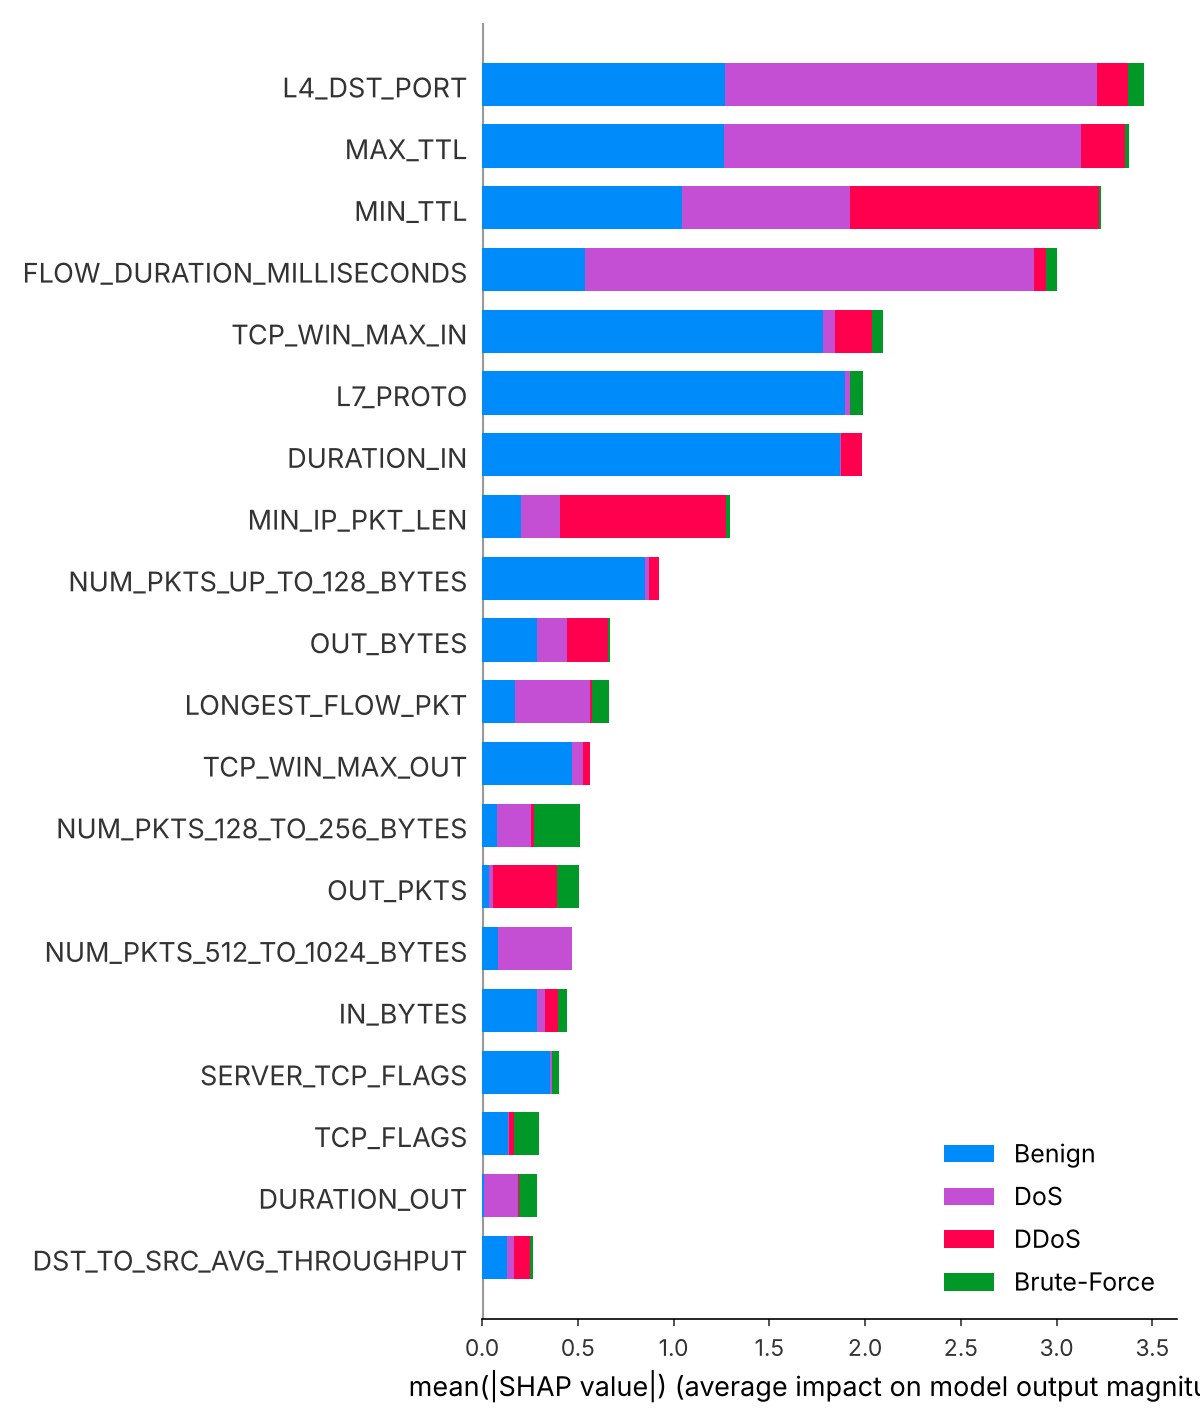
\includegraphics[width=5.8in]{assets/fig_result_shap_summary.png}
\caption{M1 SHAP summary (mean absolute Shapley value) by class, class-capped training subset, seed 42.}
\end{figure}
M1's top features by LightGBM gain importance are L4\_DST\_PORT (16.2\%), DURATION\_IN (15.3\%) and FLOW\_DURATION\_MILLISECONDS (14.0\%), followed by L7\_PROTO, MIN\_IP\_PKT\_LEN, MAX\_TTL, MIN\_TTL and TCP\_WIN\_MAX\_IN. The prominence of FLOW\_DURATION\_MILLISECONDS is notable given that Chapter 4 found this field corrupted (zero or timer-wrapped) for essentially the entire dataset; it suggests that M1 may, in part, be exploiting the field's coincidental near-binary correlation with attack type (whether a flow's duration happened to be recorded as exactly zero) rather than any genuine timing signal, which would itself be a fragile, non-generalisable basis for classification. The SHAP-based importance-share analysis used to build M5 (Table 6.4) flags exactly these two columns --- FLOW\_DURATION\_MILLISECONDS (10.7\% importance share) and DURATION\_IN (7.1\%) --- as fragile and removes them from M5's feature matrix.

\begin{table}[h]\centering
\caption{SHAP importance share of the 7 candidate timing/rate columns (M1, class-capped training subset, seed 42)}
\begin{tabularx}{\linewidth}{XXX}
\toprule
\textbf{Feature} & \textbf{Importance share} & \textbf{Flagged fragile (threshold 0.025)} \\
\midrule
FLOW\_DURATION\_MILLISECONDS & 0.1075 & Yes \\
DURATION\_IN & 0.0709 & Yes \\
DURATION\_OUT & 0.0102 & No \\
DST\_TO\_SRC\_AVG\_THROUGHPUT & 0.0095 & No \\
DST\_TO\_SRC\_SECOND\_BYTES & 0.0076 & No \\
SRC\_TO\_DST\_AVG\_THROUGHPUT & 0.0074 & No \\
SRC\_TO\_DST\_SECOND\_BYTES & 0.0052 & No \\
\bottomrule
\end{tabularx}
\end{table}
\section{Feature Importance}
\begin{table}[h]\centering
\caption{M1 top-10 features by LightGBM gain importance}
\begin{tabularx}{\linewidth}{XXX}
\toprule
\textbf{Rank} & \textbf{Feature} & \textbf{Share of total gain} \\
\midrule
1 & L4\_DST\_PORT & 16.2\% \\
2 & DURATION\_IN & 15.3\% \\
3 & FLOW\_DURATION\_MILLISECONDS & 14.0\% \\
4 & L7\_PROTO & 9.5\% \\
5 & MIN\_IP\_PKT\_LEN & 9.2\% \\
6 & MAX\_TTL & 8.1\% \\
7 & MIN\_TTL & 7.8\% \\
8 & TCP\_WIN\_MAX\_IN & 7.5\% \\
9 & LONGEST\_FLOW\_PKT & 4.0\% \\
10 & NUM\_PKTS\_128\_TO\_256\_BYTES & 2.4\% \\
\bottomrule
\end{tabularx}
\end{table}
\section{Robustness under Different Perturbation Strengths}
The project evaluates two perturbation strengths: a moderate regime (alpha \textasciitilde{} Uniform(1.5, 2.5)), which matches the range used for training-time adversarial augmentation in M4 and M5, and a stronger, out-of-distribution regime (alpha \textasciitilde{} Uniform(3.0, 4.5)), which no model ever sees during training. As Table 6.2 shows, the AER result is identical (0.00\%) at both strengths for every model; there is consequently no evidence, on this dataset, that increasing the perturbation strength from moderate to out-of-distribution changes any model's evasion resistance, because no model's resistance was ever challenged at either strength.

\section{Non-Circular SHAP Attribution-Drift Audit}
\begin{figure}[h]\centering
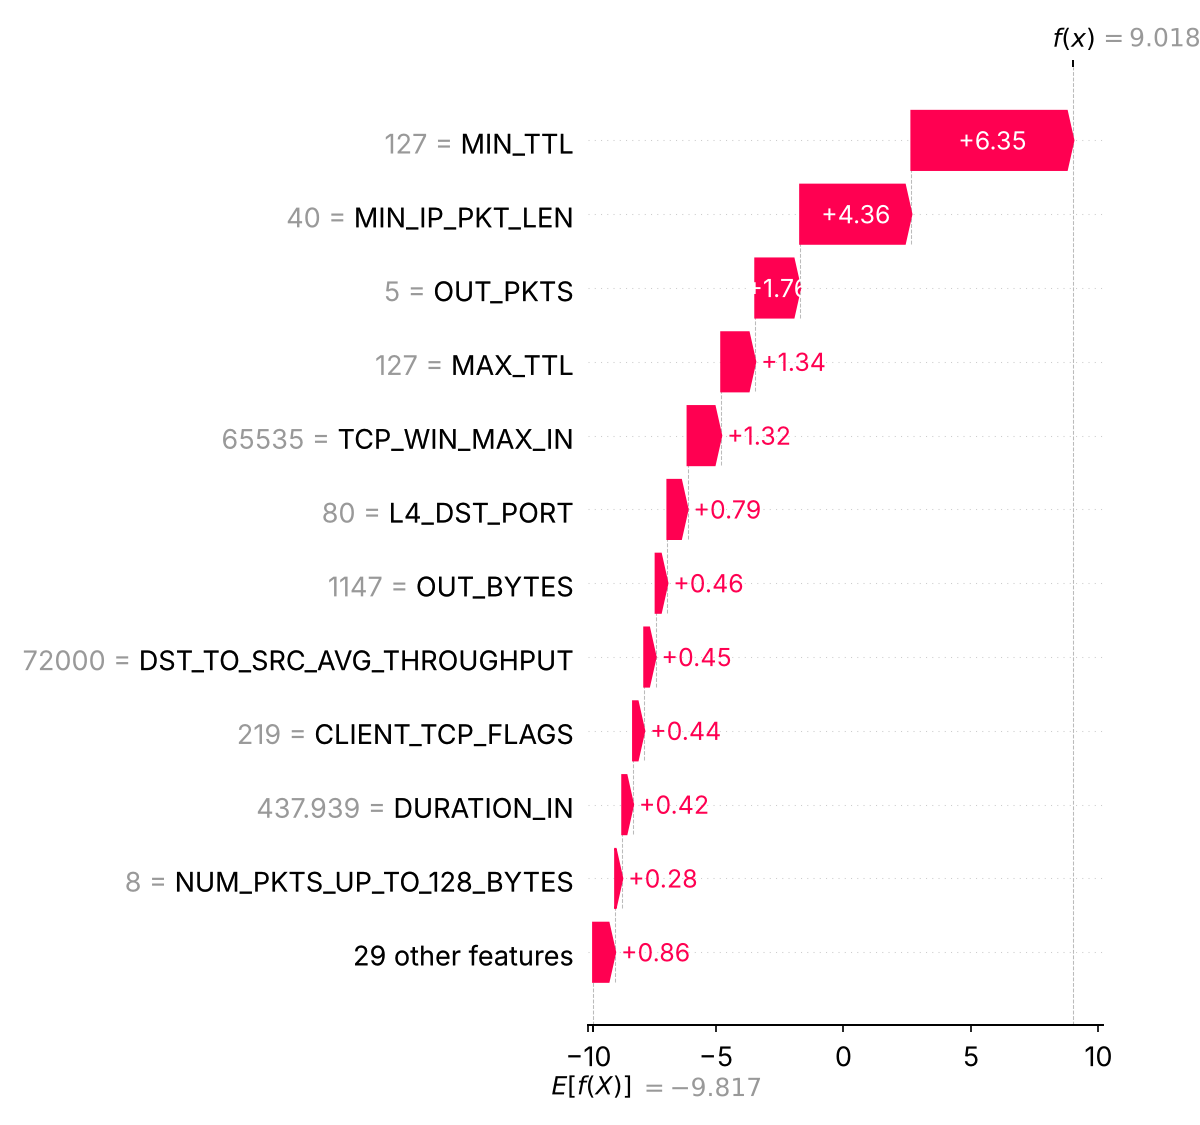
\includegraphics[width=5.8in]{assets/fig_result_waterfall_m1.png}
\caption{Representative true-class SHAP waterfall, M1, out-of-distribution perturbed flow.}
\end{figure}
\begin{figure}[h]\centering
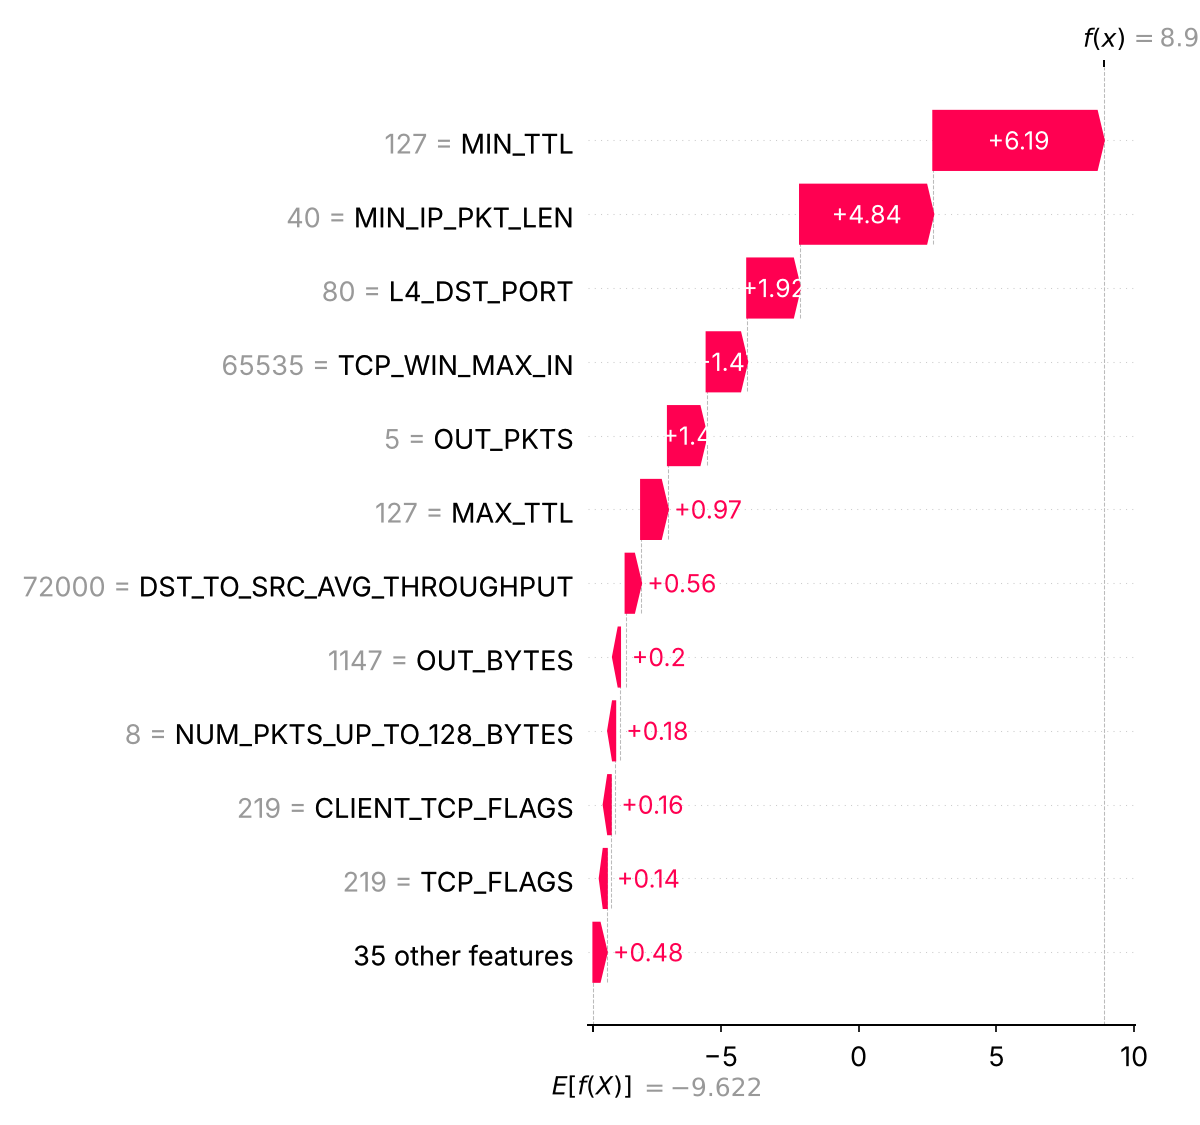
\includegraphics[width=5.8in]{assets/fig_result_waterfall_m5.png}
\caption{Representative true-class SHAP waterfall, M5, the same flow and perturbation.}
\end{figure}
The forensic audit (Section 4.10, following the project proposal's Stage 4) defines its audited flow set using only M1's own clean and out-of-distribution predictions --- never M4's or M5's --- and explains every flow for its ground-truth class, never its predicted class, so that the comparison below cannot be circular. Because the 0.00\% AER result (Section 6.2) left fewer than 30 genuinely evaded flows for every attack class, the documented fallback rule was triggered for all three classes: 300 randomly drawn clean-detected flows per class were substituted and this substitution is reported, as the project proposal requires, rather than concealed. The resulting audit set contained 649 flows.

\begin{table}[h]\centering
\caption{SHAP attribution share by feature group, on clean data, for M1, M4 and M5 (649 audited flows)}
\begin{tabularx}{\linewidth}{XXXX}
\toprule
\textbf{Model} & \textbf{Feature group} & \textbf{Features} & \textbf{Attribution share (clean)} \\
\midrule
M1 & Fragile timing/rate & 7 & 16.8\% \\
M1 & Other structural & 33 & 83.2\% \\
M4 & Fragile timing/rate & 7 & 3.8\% \\
M4 & Other structural & 33 & 96.2\% \\
M5 & Fragile timing/rate (unflagged only) & 5 & 2.7\% \\
M5 & Engineered invariant ratios & 8 & 30.7\% \\
M5 & Other structural & 33 & 66.6\% \\
\bottomrule
\end{tabularx}
\end{table}
This is the project's clearest positive finding. On clean data --- before any perturbation is applied at all --- the adversarially hardened model (M4) attributes only 3.8\% of its predictive weight to the seven fragile timing/rate features, compared with 16.8\% for the baseline (M1), a relative reduction of approximately 78\%, despite M4 having access to the exact same 40 features as M1 and differing only in its training data. The SHAP-guided hybrid model (M5) pushes this further by construction, having already removed the two most fragile columns outright, and routes a substantial 30.7\% of its attribution onto the eight engineered ratios, which are mathematically invariant under this perturbation by design. Within-model drift between each flow's clean and perturbed explanation was small for all three models (under 0.5 percentage points per group), which is itself consistent with the near-zero evasion result: there is little successfully-evaded-flow signal available to drive a larger shift. The between-model comparison on clean data, however, stands on its own: adversarial training and SHAP-guided feature engineering both measurably move predictive weight off fragile timing features, independent of whether this specific pacing attack succeeds against this specific dataset.

\section{Answering the Research Questions}
\begin{table}[h]\centering
\caption{Summary answers to the five research questions, from the evidence in this chapter}
\begin{tabularx}{\linewidth}{XXX}
\toprule
\textbf{RQ} & \textbf{Finding} & \textbf{Answer} \\
\midrule
RQ1 & M1 attributes 16.8\% of predictive weight to timing features (SHAP-confirmed reliance) but its OOD AER is 0.00\%, because no rate column could be scaled and structural features alone separate the classes & Real reliance exists; no exploitable vulnerability was demonstrated on this dataset \\
RQ2 & M2 (no timing at all) matches M1's near-ceiling clean F1 (within 0.0009) and the same 0.00\% AER & Removing timing costs almost nothing here, but cannot be shown to solve evasion that was not demonstrated \\
RQ3 & M3 and M4 reach identical clean F1 (0.9999) and identical 0.00\% AER & Inconclusive on this dataset; the SHAP audit (RQ5) is the more informative M3 vs. M4 comparison available \\
RQ4 & M5 matches M1's clean accuracy and ties M4 on AER (0.00\%) & M5 recovers accuracy with no loss, but cannot be shown to out-perform M4 on robustness that neither model was challenged on \\
RQ5 & Fragile-timing attribution share: M1 16.8\%, M4 3.8\%, M5 2.7\% (+30.7\% on engineered ratios) & Yes --- adversarial hardening and hybrid feature engineering both measurably shift predictive weight off fragile timing features \\
\bottomrule
\end{tabularx}
\end{table}
\begin{center}CHAPTER 7\end{center}
\begin{center}\textbf{CONCLUSION AND FUTURE WORK}\end{center}\vspace{4pt}
\chapter{Conclusion and Future Work}
\section{Project Summary}
This project built a complete, reproducible pipeline for studying the timing-based adversarial robustness of a flow-based NIDS: a memory-safe ingestion and sampling pipeline, an empirically-verified consistency-preserving pacing perturbation engine, a five-model comparative progression (M1--M5), and a non-circular SHAP attribution-drift audit, and executed every stage of it on the real, 17.1-million-row NF-CSE-CIC-IDS2018-v2 dataset.

\section{Major Contributions}
\begin{itemize}\setlength\itemsep{2pt}\item A two-pass, memory-safe ingestion pipeline that processes the full dataset without ever holding it in memory, with zero validation failures, zero unknown labels and zero conflicting duplicates found on the real data.\end{itemize}
\begin{itemize}\setlength\itemsep{2pt}\item A perturbation design whose rate-column scaling is gated on an empirical identity check against the real training data rather than assumed, which surfaced two genuine data-quality findings (a corrupted duration field and four unscalable rate columns) that materially shaped the experiment and are documented rather than hidden.\end{itemize}
\begin{itemize}\setlength\itemsep{2pt}\item A five-model comparative study, trained and evaluated identically across five fixed seeds, reporting clean performance and Attack Evasion Rate with full sample counts and low-support flags.\end{itemize}
\begin{itemize}\setlength\itemsep{2pt}\item A non-circular, ground-truth-class SHAP attribution-drift audit showing that adversarial hardening (M4) and SHAP-guided hybrid feature engineering (M5) both substantially reduce a LightGBM NIDS's reliance on fragile timing features --- from 16.8\% of predictive weight in the baseline to 3.8\% and 2.7\% respectively --- independent of whether the specific evasion attack evaluated succeeds.\end{itemize}
\section{Findings}
The project's two headline findings pull in different directions, and both are reported plainly, as the project's own Empirical Honesty Protocol requires. First, a negative result: the Attack Evasion Rate was 0.00\% for every model, every class, both perturbation strengths and all five seeds, because this dataset's rate/throughput columns could not be scaled under the project's own consistency criterion and because the four classes are separable almost entirely by non-timing structural features. Second, a positive result: SHAP attribution analysis shows that adversarial hardening and hybrid feature engineering both genuinely shift a model's predictive weight away from fragile timing features, which is a meaningful outcome in its own right, independent of the null evasion result.

\section{Limitations}
\begin{itemize}\setlength\itemsep{2pt}\item The dataset mirror used has a corrupted FLOW\_DURATION\_MILLISECONDS field and four rate/throughput columns that fail the project's own consistency-scaling check, which is the most likely explanation for the null AER result and limits how far RQ1, RQ3 and RQ4 can be answered on this dataset alone.\end{itemize}
\begin{itemize}\setlength\itemsep{2pt}\item The random stratified split, while deduplicated, cannot remove the effect of similar flows from the same capture campaign appearing in both training and test, since the published NetFlow schema carries no capture-day or session identifier.\end{itemize}
\begin{itemize}\setlength\itemsep{2pt}\item Bot, Infiltration and web-application attacks are out of scope by design; conclusions do not extend to them.\end{itemize}
\begin{itemize}\setlength\itemsep{2pt}\item Brute-Force contributes a small number of test flows (49 at any given seed) and its class-specific metrics, while reported in full, should be read as low-support.\end{itemize}
\begin{itemize}\setlength\itemsep{2pt}\item Reported standard deviations are computed over five seeds on one fixed sample and split, and do not capture variability from re-sampling or re-splitting the data.\end{itemize}
\section{Future Scope}
\begin{itemize}\setlength\itemsep{2pt}\item Repeat the experiment on the official, non-deduplicated UQ release of NF-CSE-CIC-IDS2018-v2, or on a different NetFlow dataset whose timing fields are not affected by exporter-level corruption, to determine whether the null AER result is specific to this dataset mirror or a more general property of NetFlow-level pacing attacks against structurally separable classes.\end{itemize}
\begin{itemize}\setlength\itemsep{2pt}\item Extend the perturbation engine to a packet-level or session-replay adversary that can also alter retransmission counters and TCP window behaviour, rather than only algebraically scaling duration and rate fields.\end{itemize}
\begin{itemize}\setlength\itemsep{2pt}\item Apply the same five-model, SHAP-guided methodology to a dataset or threat model with weaker structural separability, where a genuine timing-based evasion vulnerability is more likely to be demonstrable, to test whether M5's hybrid defence provides a measurable AER advantage over M4 when there is an actual vulnerability to recover from.\end{itemize}
\begin{itemize}\setlength\itemsep{2pt}\item Extend the non-circular SHAP audit to a larger, multi-seed audited flow set and to additional feature-group definitions, to strengthen the statistical confidence behind the RQ5 finding.\end{itemize}
\section{Potential Applications}
The methodology developed in this project --- an empirically-verified, consistency-preserving perturbation engine; a SHAP-guided feature-selection procedure targeted at robustness rather than accuracy alone; and a non-circular attribution-drift audit --- is not specific to the four attack classes studied here. It generalises directly to other flow-based intrusion-detection settings (for example, auditing a production NIDS's reliance on fields that a specific class of attacker could plausibly manipulate) and to other tabular classification settings more broadly, wherever a defender needs to know not just how accurate a model is, but what it is actually basing its decisions on, and whether a proposed defence changes that in the way it is supposed to.



% ============================================================= REFERENCES
\chapter*{References}
\addcontentsline{toc}{chapter}{References}
\begin{enumerate}[label={[\arabic*]}]
\item M. Sarhan, S. Layeghy, and M. Portmann, "Towards a Standard Feature Set for Network Intrusion Detection System Datasets," Mobile Networks and Applications, 2022, doi: 10.1007/s11036-021-01843-0 (preprint: arXiv:2101.11315).
\item M. Sarhan, S. Layeghy, N. Moustafa, and M. Portmann, "NetFlow Datasets for Machine Learning-based Network Intrusion Detection Systems," Springer, 2021 (arXiv:2011.09144).
\item NF-CSE-CIC-IDS2018-v2, Machine Learning-Based NIDS Datasets, University of Queensland. [Online]. Available: https://staff.itee.uq.edu.au/marius/NIDS\_datasets/
\item I. Sharafaldin, A. H. Lashkari, and A. A. Ghorbani, "Toward Generating a New Intrusion Detection Dataset and Intrusion Traffic Characterization," in Proc. ICISSP, 2018.
\item S. Ennaji et al., "Adversarial Challenges in Network Intrusion Detection Systems: Research Insights and Future Prospects," arXiv:2409.18736, 2024.
\item J. Vitorino, N. Oliveira, and I. Pra\c{c}a, "Adaptative Perturbation Patterns: Realistic Adversarial Learning for Robust Intrusion Detection," Future Internet, vol. 14, no. 4, art. 108, 2022 (arXiv:2203.04234).
\item G. Apruzzese, M. Andreolini, L. Ferretti, M. Marchetti, and M. Colajanni, "Modeling Realistic Adversarial Attacks against Network Intrusion Detection Systems," ACM Digital Threats: Research and Practice, 2022 (arXiv:2106.09380).
\item D. Pujol-Perich, J. Su\'arez-Varela, A. Cabellos-Aparicio, and P. Barlet-Ros, "Unveiling the potential of Graph Neural Networks for robust Intrusion Detection," ACM SIGMETRICS Performance Evaluation Review, 2022 (arXiv:2107.14756).
\item M. Rajhans and V. Khawarey, "Empirical Analysis of Adversarial Robustness and Explainability Drift in Cybersecurity Classifiers," arXiv:2602.06395, 2026 (preprint).
\item E. M. Maseno, Y. Sun, and Z. Wang, "Detecting adversarial evasion in deep learning intrusion detection systems using explainable AI," International Journal of Information Security, 2026, doi: 10.1007/s10207-026-01299-x.
\item U. Ahmed, Z. Jiangbin, A. Almogren, M. Sadiq, A. Ur Rehman, M. T. Sadiq, and J. Choi, "Hybrid bagging and boosting with SHAP based feature selection for enhanced predictive modeling in intrusion detection systems," Scientific Reports, vol. 14, art. 30532, 2024, doi: 10.1038/s41598-024-81151-1.
\item S. M. Lundberg and S.-I. Lee, "A Unified Approach to Interpreting Model Predictions," Advances in Neural Information Processing Systems (NeurIPS) 30, 2017.
\item G. Ke et al., "LightGBM: A Highly Efficient Gradient Boosting Decision Tree," Advances in Neural Information Processing Systems (NeurIPS) 30, 2017.
\item F. Pedregosa et al., "Scikit-learn: Machine Learning in Python," Journal of Machine Learning Research, vol. 12, pp. 2825--2830, 2011.
\item W. McKinney, "Data Structures for Statistical Computing in Python," in Proc. 9th Python in Science Conference (SciPy), 2010, pp. 56--61.
\item C. R. Harris et al., "Array programming with NumPy," Nature, vol. 585, pp. 357--362, 2020, doi: 10.1038/s41586-020-2649-2.
\end{enumerate}

% ============================================================= APPENDICES
\begin{center}\textbf{APPENDICES}\end{center}\vspace{4pt}
\begin{center}Appendix A: Complete Dataset Schema\end{center}
The 43 published NetFlow v9 features (3 identifiers, dropped; 40 model-input features: 33 structural + 7 timing/rate), the binary Label and the Attack class name, as defined in Chapter 4 and verified against the real downloaded file.

\begin{center}Appendix B: Original-Label to Project-Class Mapping\end{center}
See Table 4.3 (Section 4.3) for the complete, exact mapping of all 15 original Attack label strings to the 4 project classes, and the excluded labels with their reasons.

\begin{center}Appendix C: Feature Transformation Rules Under Alpha\end{center}
Duration columns (FLOW\_DURATION\_MILLISECONDS, DURATION\_IN, DURATION\_OUT): x' = alpha * x. Rate/throughput columns (SRC\_TO\_DST\_SECOND\_BYTES, DST\_TO\_SRC\_SECOND\_BYTES, SRC\_TO\_DST\_AVG\_THROUGHPUT, DST\_TO\_SRC\_AVG\_THROUGHPUT): x' = x / alpha only if empirically approved (Section 4.10); none were approved on the real dataset used in this project, so x' = x for all four. Every other model feature: x' = x (unchanged). Acceptance rule for approving a rate column: the chosen bytes/duration relationship must hold within 5\% relative error for at least 95\% of positive-duration flows.

\begin{center}Appendix D: Model Feature Matrices\end{center}
\begin{table}[h]\centering
\caption{Feature matrix size and training data for each model}
\begin{tabularx}{\linewidth}{XXXX}
\toprule
\textbf{Model} & \textbf{Input features} & \textbf{Count} & \textbf{Training rows} \\
\midrule
M1 & 33 structural + 7 timing/rate & 40 & Clean training pool (70,000) \\
M2 & 33 structural only & 33 & Clean training pool (70,000) \\
M3 & Same 40 as M1 & 40 & Clean pool + 1 Gaussian-noise copy per training attack flow \\
M4 & Same 40 as M1 & 40 & Clean pool + 1 adversarially slowed copy per training attack flow \\
M5 & 33 structural + 5 unflagged timing + 8 engineered ratios & 46 & Same augmented pool as M4 \\
\bottomrule
\end{tabularx}
\end{table}
\begin{center}Appendix E: Evaluation Metric Definitions\end{center}
Precision\_k = TP\_k / (TP\_k + FP\_k); Recall\_k = TP\_k / (TP\_k + FN\_k); F1\_k = 2 x Precision\_k x Recall\_k / (Precision\_k + Recall\_k). Clean FPR = |\{Benign test flows predicted as any attack\}| / |Benign test flows|. AER\_m = |\{flows in D\_m predicted Benign after perturbation\}| / |D\_m| x 100\%, where D\_m is the set of attack test flows model m correctly flags as non-Benign on clean data. Post-perturbation recall = |\{attack test flows predicted non-Benign after perturbation\}| / |all attack test flows|.

\begin{center}Appendix F: Reproducibility Configuration\end{center}
\begin{table}[h]\centering
\caption{Fixed experimental parameters (configs/experiment.yaml)}
\begin{tabularx}{\linewidth}{XX}
\toprule
\textbf{Parameter} & \textbf{Value} \\
\midrule
Seeds & 42, 101, 202, 303, 404 \\
Sample size & 100,000 flows \\
Train/test split & 70\% / 30\%, stratified, seed 42 \\
Chunk size & 200,000 rows \\
Model & LGBMClassifier(class\_weight='balanced'), n\_estimators=300, learning\_rate=0.1, num\_leaves=31, subsample=0.8, subsample\_freq=1, colsample\_bytree=0.8 \\
M3 noise sigma & 0.10 (fraction of each feature's training standard deviation) \\
Training augmentation alpha range & Uniform(1.5, 2.5) \\
Moderate test alpha range & Uniform(1.5, 2.5) \\
Out-of-distribution test alpha range & Uniform(3.0, 4.5) \\
SHAP fragility threshold & 1/40 = 0.025 (sensitivity also reported at 0.01 and 0.05) \\
SHAP selection subset cap & 2,500 flows per class \\
SHAP audit cap & 300 flows per true class \\
\bottomrule
\end{tabularx}
\end{table}
\begin{center}Appendix G: List of Project Output Files\end{center}
schema\_verification.csv, label\_mapping\_log.csv, class\_counts.csv, validation\_drops.csv, duplicate\_conflicts.csv, sampling\_quotas.csv, sample\_100k.parquet, train.parquet, test.parquet, shap\_selection.csv, m5\_feature\_list.json, shap\_summary\_m1.png, perturbed\_moderate\_seed*.parquet, perturbed\_ood\_seed*.parquet, perturbation\_consistency\_check.csv, clean\_metrics\_summary.csv, metrics\_moderate.csv, metrics\_ood.csv, aer\_by\_class.csv, aer\_summary.csv, confusion matrices (per model, per seed), shap\_drift\_table.csv, shap\_drift\_group\_summary.csv, audit\_sample\_ids.csv, shap\_waterfall\_m1.png, shap\_waterfall\_m5.png, run\_config.json, results\_summary.md.



\end{document}
